\documentclass{article}
\usepackage[dblblindworkshop]{neurips_2026}
\workshoptitle{Machine Learning and the Physical Sciences (ML4PS)}
\usepackage[utf8]{inputenc}
\usepackage[T1]{fontenc}
\usepackage{amsmath}
\usepackage{amssymb}
\usepackage{booktabs}
\usepackage{graphicx}
\usepackage{microtype}
\usepackage{xcolor}
\usepackage{url}
\usepackage{hyperref}
\usepackage{multirow}
\usepackage{array}
\usepackage{enumitem}
\usepackage{placeins}
\newcommand{\method}{AstroJEPA}
\newcommand{\prealign}{Pretrain$\rightarrow$Align}
\newcommand{\joint}{Joint-Scratch}
\newcommand{\rscore}{$R^2$}
\setlength{\bibsep}{2pt plus 0.3ex}
\setlist[itemize]{leftmargin=*,topsep=2pt,itemsep=1pt,parsep=0pt}

\title{\method: Cross-Modal Joint-Embedding Learning\\
for Astronomical Images and Spectra}
\author{Anonymous Authors}

\begin{document}
\maketitle

\begin{abstract}
Images and spectra record complementary views of the same galaxy, yet most
astronomical representation models either learn each modality separately or
align them with contrastive negatives.
We introduce \method, a teacher-free joint-embedding framework that matches
augmented image and spectrum views while Sketched Isotropic Gaussian
Regularization (SIGReg) prevents collapse.
We ask how \method\ should be trained: align frozen unimodal encoders through
learned poolers, or learn both encoders jointly from random initialization.
On 307,428 DESI--Legacy Survey pairs, joint training improves every tested
physical-property probe in the shared space, raises cross-modal CKA from
0.720 to 0.770 and mean bidirectional recall@10 from 0.87\% to 2.97\%, and
more than doubles shared effective rank.
Raw joint backbones retain modality-specific information, including image
morphology that the shared projection filters out.
A matched contrastive baseline retrieves exact pairs better but is less
globally transformable, showing that \method's principal value is a useful,
non-collapsed shared scientific representation rather than instance matching
alone.
\end{abstract}

\section{Introduction}
\label{sec:intro}

Modern sky surveys observe the same object through complementary sensors.
Galaxy images encode projected light and morphology; spectra expose redshift,
stellar populations, and emission lines.
A representation that connects these channels could support cross-survey
search, cross-modal imputation, and physical inference with fewer labels.
Existing astronomy foundation models have demonstrated the value of large-scale
unimodal pretraining and contrastive image--spectrum alignment
\citep{parker2024astroclip,parker2025aion}.
The open question is whether explicit negative pairs are necessary to learn a
scientifically useful joint space.

Joint-embedding predictive architectures (JEPAs) learn invariances in latent
space rather than reconstructing pixels \citep{assran2023ijepa}.
LeJEPA makes this recipe teacher-free by combining an invariance term with
SIGReg, which regularizes random one-dimensional projections toward an
isotropic Gaussian \citep{balestriero2025lejepa}.
We adapt that principle across modalities.
\method\ maps two augmented views of a galaxy image and two masked/noisy views
of its spectrum to a 256-dimensional shared space, matches all four
cross-modal view pairs, and applies SIGReg separately to each branch.
It uses no negatives, queue, EMA teacher, stop-gradient target, reconstruction,
or within-modality loss.

Our central experiment compares two practical ways to obtain \method\
(Figure~\ref{fig:architecture}): (i) independently pretrain the image and
spectrum encoders, freeze them, and align learned-query poolers; or (ii) train
both encoders and projectors jointly from scratch.
This is deliberately a \emph{strategy comparison}, not an initialization-only
ablation: the completed systems differ in trainable capacity and duration.
We then ask what alignment preserves or removes, and use a controlled
contrastive run only as a secondary objective baseline.

The paper makes three contributions:
\begin{itemize}
    \item \textbf{A cross-modal JEPA framework for astronomy.} We specify and
    validate a non-collapsed, end-to-end image--spectrum model on 307k pairs.
    \item \textbf{A training-strategy study.} Joint learning consistently
    outperforms the implemented frozen-pooler route in scientific probes,
    retrieval, cross-modal geometry, and effective rank.
    \item \textbf{A representation audit.} Raw backbones retain useful
    modality-private information that shared projections intentionally filter;
    detailed CLIP comparisons and all supporting diagnostics are reported in
    Appendices~\ref{app:strategy}--\ref{app:figures}.
\end{itemize}

\section{\method}
\label{sec:method}

\begin{figure}[t]
  \centering
  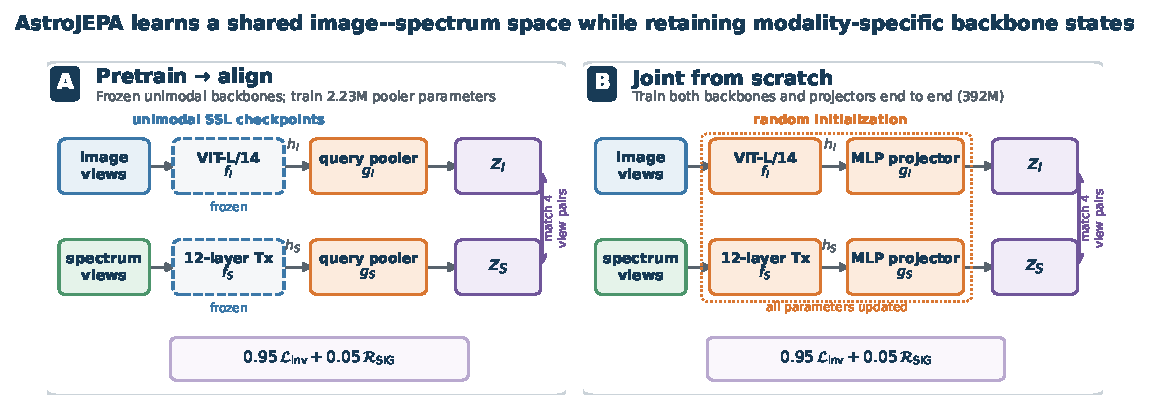
\includegraphics[width=\linewidth]{Figures/astrojepa_architecture.pdf}
  \caption{\textbf{\method\ and the two training strategies.}
  Both routes expose raw modality states $h_I,h_S$ and learn shared states
  $z_I,z_S$ with the same cross-modal invariance--SIGReg objective.
  \prealign\ freezes independently trained backbones and updates two
  learned-query poolers; \joint\ learns encoders and MLP projectors end to end.
  Dashed blue boxes are frozen and orange boxes are trainable.
  Full architectures and objectives are in Appendix~\ref{app:architecture}.}
  \label{fig:architecture}
\end{figure}

\paragraph{Encoders and objective.}
The image branch is a ViT-L/14 with 1,024-dimensional raw output; the spectrum
branch is a 12-layer, 768-dimensional transformer over 389 non-overlapping
20-pixel patches.
Modality-specific heads map to $z_I,z_S\in\mathbb R^{256}$.
For two image views $x_I^{(v)}$ and two spectrum views $x_S^{(u)}$,
\begin{equation}
\mathcal L_{\rm AJ}
=0.95\,\frac{1}{4}\sum_{v=1}^{2}\sum_{u=1}^{2}
\left\lVert z_I^{(v)}-z_S^{(u)}\right\rVert_2^2
+0.05\,\frac{\mathcal R_{\rm SIG}(z_I)+
\mathcal R_{\rm SIG}(z_S)}{2}.
\label{eq:astrojepa}
\end{equation}
SIGReg uses 1,024 random slices and 17 evaluation points.
The unnormalized embeddings enter both terms; normalization is used only for
cosine evaluation.
Although motivated by the JEPA family, the implemented cross-modal loss is
direct latent invariance rather than masked predictor-based I-JEPA.

\paragraph{Two training strategies.}
\prealign\ starts from an image ViT-L pretrained on 8.47M galaxies and a
spectrum transformer pretrained on 1.10M DESI spectra.
Both backbones remain frozen; AstroCLIP-style learned-query attention poolers
contribute 2.23M trainable parameters and are optimized for 10 epochs
(24k updates).
\joint\ randomly initializes both branches and updates the full 392M-parameter
system for 50 epochs (60k updates).
Both see the same 307,428 paired objects and use AdamW at $10^{-4}$, but
\prealign\ uses global batch 128 whereas \joint\ uses 256.
Accordingly, our conclusion is restricted to the two completed strategies;
a matched full-finetuning control remains necessary.

\section{Experiments}
\label{sec:experiments}

\paragraph{Data and evaluation.}
The 307,428-pair corpus comprises 197,976 AstroCLIP-mirror objects,
95,895 DESI--Legacy DR10 matches, and 13,557 new DESI--DR8 matches
\citep{desi2024edr,dey2019legacy}.
We evaluate on the 168,280-object mirror with its historical
138,583/29,697 train/test split.
Physical probes use the 89,334-object PROVABGS subset
\citep{hahn2023provabgs}; retrieval uses every one of the 29,697 test
candidates.
Because representation training consumed all 307k unlabeled pairs, including
mirror test identities, the evaluation is transductive: probe heads and maps
are held out, but the objects are not.
Appendices~\ref{app:data}--\ref{app:training} give preprocessing, schedules,
hardware, and split details.

\subsection{AstroJEPA learns scientifically useful shared representations}
\label{sec:utility}

\begin{table}[h!]
\centering
\caption{\textbf{Frozen ridge-probe \rscore\ on shared 256-d \method\
representations.} Joint training improves all five properties for both
modalities. Values are means over three probe seeds; standard deviations are
below $8\times10^{-4}$.}
\label{tab:main_probes}
\small
\setlength{\tabcolsep}{4.3pt}
\begin{tabular}{llccccc}
\toprule
Training & View & Redshift & Mass & Metal. & Age & sSFR \\
\midrule
\prealign & Image    & .512 & .672 & .401 & .210 & .498 \\
          & Spectrum & .574 & .715 & .427 & .254 & .533 \\
\joint    & Image    & \textbf{.613} & \textbf{.768} & \textbf{.459} & \textbf{.278} & \textbf{.564} \\
          & Spectrum & \textbf{.632} & \textbf{.780} & \textbf{.448} & \textbf{.274} & \textbf{.570} \\
\bottomrule
\end{tabular}
\end{table}

Table~\ref{tab:main_probes} establishes the first requirement of a shared
scientific space: both modalities linearly expose redshift and four
stellar-population properties.
The spectrum branch is strongest, as expected from the measurement channel,
but image embeddings also encode every target.
\joint\ improves mean probe \rscore\ from 0.459 to 0.537 for images and from
0.500 to 0.541 for spectra.
Its raw backbones are stronger still (mean 0.562 image and 0.614 spectrum),
showing that the shared head is a selective interface rather than a replacement
for modality-specific features.

\subsection{Joint learning outperforms frozen-pooler alignment}
\label{sec:strategy}

\begin{figure}[h!]
  \centering
  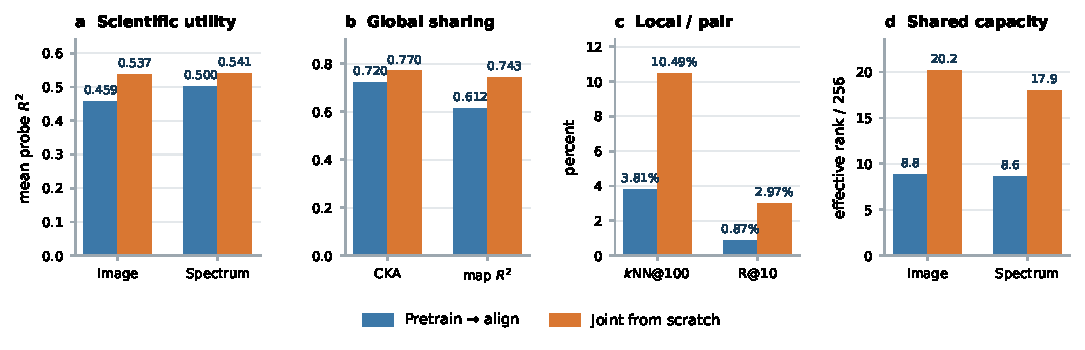
\includegraphics[width=\linewidth]{Figures/astrojepa_training_comparison.pdf}
  \caption{\textbf{The implemented joint strategy wins across complementary
  criteria.} Scientific utility averages the five shared-space probes in
  Table~\ref{tab:main_probes}; map \rscore\ and recall@10 are bidirectional
  means. CKA uses all 168,280 objects, while neighborhood overlap and retrieval
  use the 29,697-object test pool. Effective rank is computed from the
  256-dimensional shared states.}
  \label{fig:training}
\end{figure}

The advantage is not confined to downstream labels
(Figure~\ref{fig:training}).
\joint\ raises cross-modal linear CKA from 0.720 to 0.770 and bidirectional
ridge-map \rscore\ from 0.612 to 0.743.
Exact cross-modal neighborhood overlap at $k=100$ increases from 3.81\% to
10.49\%, and bidirectional recall@10 from 0.87\% to 2.97\%.
The sequential shared states occupy a narrow manifold---effective rank
8.83/8.60 for image/spectrum---whereas the joint states reach 20.19/17.94.
Thus the end-to-end route is simultaneously more useful, more mutually
predictable, and less dimensionally concentrated.
These consistent outcomes motivate joint training as our default \method\
recipe, while the capacity and optimization confound prevents claiming that
unimodal pretraining itself is harmful.

\subsection{What changes during cross-modal learning?}
\label{sec:change}

The raw joint encoders are not simple copies of the independent ones:
same-modality CKA is 0.451 for images and 0.398 for spectra; neighborhood
overlap@100 is 14.3\% and 7.5\%.
Yet the image backbone retains morphology.
On Galaxy10 \citep{leung2024galaxy10}, its frozen linear probe reaches
$72.22\pm1.26$\% accuracy and $70.19\pm1.30$\% macro-F1, matching the
independent image encoder's $71.83\pm0.84$\% and
$70.23\pm0.90$\%.
The joint shared image projection falls to
$44.99\pm0.97$\% accuracy.
The common bottleneck therefore filters image-private morphology even while
the backbone preserves it.

Cross-modal ridge prediction provides a complementary shared/private audit.
For the joint model, the image-predictable part of the spectrum has mean probe
\rscore\ 0.531 versus 0.535 for the total spectrum state; its residual still
scores 0.107.
The spectrum-predictable image component scores 0.534 versus 0.531 total,
with residual 0.071.
This is a linear decomposition, not mutual information: residuals also contain
nonlinear shared structure and mapping error.
The result nevertheless supports exposing both $(z_m,h_m)$ rather than only a
single common vector.

\subsection{A compact contrastive control}
\label{sec:clip}

We also train CLIP from random initialization for the same 50 epochs, paired
objects, architectures, and views \citep{radford2021clip}.
CLIP improves bidirectional recall@10 from 2.97\% to 7.98\%, but \method\ has
higher projected CKA (0.770 vs.\ 0.634), pairwise-geometry correlation
(0.607 vs.\ 0.485), and bidirectional linear-map \rscore\
(0.749/0.736 vs.\ 0.551/0.549).
This result bounds the claim: \method\ does not dominate exact instance
matching; it learns a more globally congruent and linearly transformable shared
space under these runs.
The full comparison---raw and projected probes, CCA, Procrustes retrieval,
decoder transfer, eigenspectra, and all plots---is intentionally moved to
Appendix~\ref{app:clip}.

\section{Discussion}
\label{sec:discussion}

A frozen pooler must discover the intersection of two independently organized
token spaces, whereas paired end-to-end gradients can reorganize both
encoders.
The sequential ranks near nine are consistent with a narrow intersection but
do not prove this mechanism because head and budget also change.
Contrastive negatives sharpen instance ranking, while AstroJEPA's invariance
makes modalities more linearly transformable; neither property alone captures
quality.
For science, the shared state can support retrieval and cross-modal prediction,
while the raw state retains channel-specific morphology or spectral detail.
Exposing both makes information discarded by alignment measurable.

\section{Limitations and impact}
\label{sec:limitations}

Each principal representation has one training seed, so deterministic
full-pool diagnostics do not quantify training-seed variance.
The strategies also differ in parameters, duration, batch, and head type.
Evaluation is transductive and DESI-dominated; retrieval counts valid analogues
and duplicates as errors.
A definitive test needs object-disjoint pretraining, matched full-model
fine-tuning, multiple seeds, and a no-SIGReg control.

\method\ may reduce labeling needs and enable large-catalog search or
cross-modal imputation, but it inherits survey selection, calibration,
cross-match, and physical-label biases.
Embeddings are not calibrated physical estimators and require downstream
validation.
The data are public astronomical observations and contain no personal data;
the main concern is compute and the risk of overconfident scientific use.

\paragraph{Conclusion.}
\method\ learns useful shared image--spectrum representations without
contrastive negatives.
For the completed systems, joint training is strongest, while raw states
preserve science filtered by the common bottleneck.

\clearpage
\bibliographystyle{plainnat}
\bibliography{references}

\clearpage
\appendix

\section{Full \method\ Architecture and Objectives}
\label{app:architecture}

\subsection{Terminology and scope}

We use \emph{AstroJEPA} for the complete image--spectrum representation
framework, and \emph{JEPA+SIGReg} when naming its optimization objective in
control tables.
The system follows the joint-embedding principle---predict or match targets in
representation space rather than reconstructing inputs---and uses LeJEPA's
teacher-free distributional regularization.
It is not the canonical masked-image I-JEPA architecture: there is no context
encoder, EMA target encoder, predictor, or stop-gradient branch.
This distinction matters because Equation~\ref{eq:astrojepa} is direct
cross-modal invariance.

\subsection{Backbones and heads}

\begin{table}[h]
\centering
\caption{Architecture used by the completed cross-modal runs.}
\label{tab:architecture}
\small
\setlength{\tabcolsep}{5pt}
\begin{tabular}{p{0.16\linewidth}p{0.34\linewidth}ccc}
\toprule
Branch & Encoder & Raw dim. & Tokens & Shared dim.\\
\midrule
Image & ViT-L/14, 24 blocks, 16 heads & 1,024 & $10\times10+1$ & 256\\
Spectrum & Transformer, 12 blocks, 12 heads, MLP ratio 4 & 768 & $389+1$ & 256\\
\bottomrule
\end{tabular}
\end{table}

The image encoder consumes 140$\times$140 three-channel astronomy images.
The spectrum encoder consumes a fixed 7,781-pixel DESI grid.
It retains the first 7,780 pixels as 389 disjoint patches of width 20 and adds
a CLS token.
A patch is attendable when at least half of its pixels are scientifically
valid; invalid padding, physical masks, and artificial augmentation masks
remain distinct.

In \joint, each CLS state enters a modality-specific MLP projector.
In \prealign, token sequences enter independent learned-query cross-attention
poolers with four attention heads, dropout 0.1, a residual connection, and a
fourfold-width MLP; the frozen image and spectrum tensors are not copied into
the alignment checkpoint.
Total parameters are 391,990,528, of which 2,234,368 are trainable in
\prealign\ and approximately 392M in \joint.

\subsection{Cross-modal AstroJEPA loss}

Let $B$ be the local batch and $V_I=V_S=2$.
For each object, Equation~\ref{eq:astrojepa} averages all
$V_I V_S=4$ squared-error pairs.
SIGReg applies independent random projections to the image and spectrum
embedding batches:
\[
\mathcal R_{\rm SIG}
=\frac{1}{K}\sum_{k=1}^{K}
\operatorname{EP}\!\left(\{\langle z_b,\theta_k\rangle\}_{b=1}^{B},
\mathcal N(0,1)\right),
\qquad K=1024,
\]
where $\operatorname{EP}$ is the Epps--Pulley normality statistic evaluated at
17 points.
Random slice seeds and differentiable distributed moments are synchronized
across ranks.
The regularizer sees the effective distributed batch without requiring a full
embedding all-gather.
No image--image, spectrum--spectrum, local-patch, reconstruction, contrastive,
or distillation term is active in the completed cross-modal runs.

\subsection{Independent unimodal objectives}

The image SSL model receives two 140-pixel global crops and eight 56-pixel local
crops.
Its invariance target is the mean of the two global projected states and its
loss is $0.95\,\mathcal L_{\rm view}+0.05\,\mathcal R_{\rm SIG}$.
The 1,024-dimensional ViT-L state is followed during training by a
1,024--2,048--2,048--64 projector; downstream evaluation normally uses the raw
backbone.

Spectrum SSL receives two independently masked and noise-perturbed views and
optimizes
\[
\mathcal L_{\rm spec}
=\underbrace{0.95\mathcal L_{\rm CLS}+0.05\mathcal R_{\rm SIG}^{\rm global}}
_{\mathcal L_{\rm global}}
+\underbrace{0.95\mathcal L_{\rm patch}
+0.05\mathcal R_{\rm SIG}^{\rm local}}_{\mathcal L_{\rm local}} .
\]
Patch comparisons use the same wavelength positions and exclude invalid
targets.
The 768-dimensional raw state and 64-dimensional objective head are both
evaluated in Appendix~\ref{app:unimodal}.

\subsection{Contrastive control}

The secondary scratch CLIP control uses the same encoders, projectors, paired examples,
and four view combinations as \joint.
It $\ell_2$-normalizes projected embeddings and averages symmetric
image-to-spectrum and spectrum-to-image InfoNCE.
Differentiable all-gather supplies every object in the global batch as a
candidate.
Temperature is learned from 0.07 and the multiplicative logit scale is capped
at 100.
SIGReg and same-modality terms are absent.
A separate frozen-backbone control uses the same learned-query topology as
\prealign, a 512-dimensional output, fixed logit scale 15.5, and global-batch
InfoNCE; its results are isolated in Appendix~\ref{app:clip}.

\FloatBarrier
\section{Data and Preprocessing}
\label{app:data}

\subsection{Corpus inventory}

\begin{table}[h]
\centering
\caption{Datasets used for representation training and evaluation. Counts are
objects after the stated local filtering; Galaxy10 DECaLS is from
\citet{leung2024galaxy10}.}
\label{tab:data_inventory}
\small
\begin{tabular}{p{0.35\linewidth}rp{0.42\linewidth}}
\toprule
Dataset & Objects & Role\\
\midrule
Smith42/galaxies & 8,474,566 & streamed image SSL\\
DESI EDR/SV3 spectra & 1,126,441 & spectrum SSL; 1,103,874 train\\
Paired DESI--Legacy union & 307,428 & cross-modal representation training\\
AstroCLIP benchmark mirror & 168,280 & maps, retrieval, redshift probes\\
PROVABGS valid subset & 89,334 & four stellar-population probes\\
Galaxy10 DECaLS & 17,736 & 10-way morphology\\
\bottomrule
\end{tabular}
\end{table}

The spectrum SSL object-ID split contains 1,103,874 train, 11,280 validation,
and 11,287 test spectra.
The evaluation mirror retains its historical 138,583/29,697 split.
After requiring valid PROVABGS labels, 73,341 objects remain in train and
15,993 in test.
Galaxy10 uses three stratified 80/10/10 splits; checkpoint selection uses
validation macro-F1.

\begin{table}[h]
\centering
\caption{Composition and harmonization of the 307,428-pair corpus.}
\label{tab:pair_sources}
\small
\setlength{\tabcolsep}{4pt}
\begin{tabular}{lrrp{0.42\linewidth}}
\toprule
Source & Rows & Fraction & Model-facing contract\\
\midrule
AstroCLIP mirror & 197,976 & 64.40\% & flux-only DESI; raw $g/r/z$ nanomaggies\\
MMU DESI--DR10 & 95,895 & 31.19\% & flux/ivar/mask; rendered RGB PNG\\
Manual DESI--DR8 & 13,557 & 4.41\% & flux/ivar/mask; DR8 crop\\
\midrule
Total & 307,428 & 100\% & fixed spectrum grid; two 140-pixel image views\\
\bottomrule
\end{tabular}
\end{table}

The manual cross-match initially contained 13,579 new target IDs; 21 missing
image IDs removed 22 pair rows during materialization.
No spectrum payload was missing.
AstroCLIP nanomaggy images use the published $g/r/z$ arcsinh RGB mapping before
common augmentations.
Every spectrum is mapped to the same 7,781-pixel grid and normalized by its
valid-pixel mean and standard deviation.
MMU/manual rows retain pipeline inverse variance and masks; flux-only
AstroCLIP rows mark finite values valid and disable uncertainty noise rather
than synthesizing inverse variance.

\subsection{Augmentations}

Images use random resized crops, horizontal/vertical flips, rotations, and
astronomy-specific blur/noise transforms.
Independent image SSL uses two 140-pixel global and eight 56-pixel local views;
cross-modal training uses two 140-pixel global views.
Spectra use two views with 30\% disjoint span masks, span length 2--12 patches,
and inverse-variance-scaled Gaussian noise with scale 0.5 capped at normalized
standard deviation 3.
Positive inverse variance determines augmentation noise but is not an encoder
channel or loss weight.
Wavelength is implicit in fixed token position; wavelength and line-spread
function are validated metadata, and LSF is not yet an input.

\subsection{Evaluation leakage boundary}

Cross-modal SSL intentionally uses all available pairs without historical
split labels.
Consequently, representations may have seen the unlabeled identity of objects
later used in the mirror test set.
All ridge probes, cross-modal maps, and hyperparameter selection remain
train-only, but this does not make the backbone test object-disjoint.
We therefore use these results for controlled representation comparison and do
not present them as strict unseen-object generalization.

\FloatBarrier
\section{Training and Evaluation Details}
\label{app:training}

\begin{table}[h]
\centering
\caption{Completed principal training runs. Samples counts source-object
presentations, not augmented views.}
\label{tab:training_runs}
\scriptsize
\setlength{\tabcolsep}{3.3pt}
\begin{tabular}{lrrrrrr}
\toprule
Run & Trainable & GPUs & Global batch & Epochs & Updates & Samples\\
\midrule
Image SSL ViT-L & 310.8M & 4 & 768 & 5 passes & 54,940 & 42.19M\\
Spectrum SSL v2 & 87M & 4 & 64 & 10 & 172,390 & 11.04M\\
\prealign & 2.23M & 4 & 128 & 10 & 24,000 & 3.07M\\
Frozen InfoNCE & 7.09M & 4 & 256 & 10 & 12,000 & 3.07M\\
\joint & $\sim$392M & 4 & 256 & 50 & 60,000 & 15.36M\\
CLIP scratch & $\sim$392M & 4 & 128 & 50 & 120,000 & 15.36M\\
\bottomrule
\end{tabular}
\end{table}

All four cross-modal configurations use AdamW with learning rate $10^{-4}$, weight decay
0.05, 1,000 warmup updates, cosine decay to $10^{-6}$, bfloat16, gradient-norm
clipping at 1, and seed 42.
\joint\ ran for 10 h 13 min and CLIP for 11 h 5 min on four GPUs.
They match architectures, views, epochs, sample exposure, and approximately
wall time, but not global batch or update granularity.
The frozen \prealign\ run uses the same optimizer family and paired corpus but
is intentionally shorter.

Image SSL uses AdamW at $5\times10^{-4}$, weight decay 0.05, 1,000-step
warmup, cosine decay to $10^{-6}$, and bfloat16.
The five streamed passes correspond to 42.19M source-image presentations and
421.94M augmented views.
Spectrum v2 uses the same optimizer values and numerical settings for ten true
passes.
Its corrected schedule is 17,239 synchronized updates per epoch.

\paragraph{Frozen probes.}
Continuous targets are standardized from the training set.
Ridge regularization is selected on a train-only validation carve-out and the
model is refit on the remaining training rows.
Reported values average three deterministic split seeds.
Galaxy10 uses a class-balanced linear classifier; accuracy and macro-F1 are
means and standard deviations over three stratified splits.

\paragraph{Alignment diagnostics.}
Exact retrieval ranks every candidate by cosine similarity.
Cross-modal $k$NN overlap is
$|N_k^I(x)\cap N_k^S(x)|/k$, averaged over queries.
Linear CKA uses centered Gram matrices.
Pairwise geometry samples 500,000 deterministic object pairs and correlates
within-modality cosine similarities with Spearman's $\rho$.
Cross-modal ridge maps select their penalty on training data and report held-out
global \rscore.
CCA, orthogonal Procrustes, covariance eigenspectra, participation ratio, and
effective rank provide complementary subspace diagnostics.

\FloatBarrier
\section{Independent Unimodal SSL}
\label{app:unimodal}

\subsection{Image SSL}

\begin{table}[h]
\centering
\caption{Controlled Galaxy10 frozen linear probes.}
\label{tab:image_galaxy10}
\small
\begin{tabular}{lrrr}
\toprule
Backbone & Selected update & Accuracy (\%) & Macro-F1 (\%)\\
\midrule
ResNet9 & 8,000 & $44.80\pm1.75$ & $42.69\pm1.70$\\
ViT-S/14 & 21,000 & $61.19\pm1.42$ & $59.34\pm1.16$\\
ViT-L/14 & 52,000 & $\mathbf{71.83\pm0.84}$ & $\mathbf{70.23\pm0.90}$\\
\bottomrule
\end{tabular}
\end{table}

The ViT-L has 304.37M backbone parameters and 6.43M projector parameters.
A two-layer MLP probe reached approximately 72.4\% accuracy, only a small gain
over the linear head.
The recorded DINOv2 ViT-g/14 and AION-1-L contexts are 71.4\% and 87.2\%,
respectively \citep{oquab2023dinov2,parker2025aion}; these use different
pretraining, data, and downstream heads and are not a matched leaderboard.

\begin{table}[h]
\centering
\caption{Fixed-seed image-redshift \rscore\ over the ViT-L checkpoint series.
The broad late plateau motivated selecting update 52k by Galaxy10 validation
macro-F1 rather than redshift test performance.}
\label{tab:image_redshift_series}
\scriptsize
\setlength{\tabcolsep}{3.0pt}
\begin{tabular}{lrrrrrrrr}
\toprule
Update (k) & 4 & 8 & 12 & 16 & 20 & 24 & 28 & 32\\
\midrule
\rscore & .51761 & .52786 & .52551 & .52723 & .52938 & .53032 & .53033 & .53018\\
\midrule
Update (k) & 36 & 40 & 44 & 48 & 52 & 54.94 & CPT 62.99 & AstroDINO\\
\midrule
\rscore & .53117 & \textbf{.53167} & .53137 & .53089 & .53028 & .53023 & .53128 & .52888\\
\bottomrule
\end{tabular}
\end{table}

The one-epoch local-data continuation improves its 52k source by only about
0.001 \rscore.
The historical Galaxy10 redshift probe reports 0.748 after restricting to
$z<0.25$; it is a different sample and is not compared numerically with the
DESI--Legacy mirror.

\subsection{Spectrum SSL}

\begin{table}[h]
\centering
\caption{Frozen spectrum probe \rscore. V2 is the corrected global+local
LeJEPA run; projected is its 64-dimensional objective head.}
\label{tab:spectrum_ssl}
\small
\setlength{\tabcolsep}{5pt}
\begin{tabular}{lccccc}
\toprule
Representation & Redshift & Mass & Metal. & Age & sSFR\\
\midrule
Spectrum v1 raw & .432 & .506 & .235 & .185 & \textbf{.510}\\
Spectrum v2 raw & \textbf{.555} & \textbf{.698} & \textbf{.409} & \textbf{.232} & .496\\
Spectrum v2 projected & .388 & .541 & .259 & .104 & .430\\
\bottomrule
\end{tabular}
\end{table}

V2 improves four of five raw targets substantially but slightly regresses
sSFR.
Its raw effective rank is 13.67/768 (participation ratio 9.59, largest
eigenvalue share 0.208); the 64-dimensional projector has effective rank
23.03 (participation ratio 17.36, largest share 0.117).
The lower projected probe scores reinforce the practice of using the backbone,
not the SSL head, for unimodal science.

\begin{table}[h]
\centering
\caption{Linear and two-layer MLP probes on the \joint\ raw spectrum state.
The nonlinear head principally helps redshift and age.}
\label{tab:nonlinear}
\small
\begin{tabular}{lccccc}
\toprule
Probe & Redshift & Mass & Metal. & Age & sSFR\\
\midrule
Ridge & .676 & .843 & .549 & .366 & .639\\
Two-layer MLP & $.702\pm.003$ & .854 & .580 & $.410\pm.004$ & .668\\
\bottomrule
\end{tabular}
\end{table}

The earlier 95k-pair scratch pilot reached raw spectrum \rscore\
0.642/0.823/0.533/0.321/0.629 (redshift/mass/metallicity/age/sSFR), but its
loader under-consumed rows per nominal epoch.
Its image redshift scores were .523 raw and .517 shared; raw effective rank was
9.64/7.04 for image/spectrum and shared rank was 8.58/10.07.
Its spectrum shared scores were .588/.775/.443/.249/.588 in the same target
order.
It is retained as 8,396-update feasibility evidence, not as a controlled
50-epoch result.

The dedicated unimodal battery and the later strategy-study cache give slightly
different values after their respective evaluation pipelines (for example,
spectrum-v2 mass .698 here and .695 in Table~\ref{tab:full_strategy_probes}).
All within-strategy conclusions use one pipeline consistently.

\clearpage
\section{Cross-Modal Training: Pretrained vs.\ Scratch}
\label{app:strategy}

\subsection{Complete downstream probes}

\begin{table}[h]
\centering
\caption{All frozen ridge-probe \rscore\ for the two \method\ strategies.
Raw is the backbone state; shared is the objective-facing 256-d state.}
\label{tab:full_strategy_probes}
\scriptsize
\setlength{\tabcolsep}{3.6pt}
\begin{tabular}{lllccccc}
\toprule
Training & Modality & State & Redshift & Mass & Metal. & Age & sSFR\\
\midrule
\multirow{4}{*}{\prealign}
& Image & raw & .530 & .691 & .413 & .241 & .501\\
& Image & shared & .512 & .672 & .401 & .210 & .498\\
& Spectrum & raw & .555 & .695 & .409 & .228 & .496\\
& Spectrum & shared & .574 & .715 & .427 & .254 & .533\\
\midrule
\multirow{4}{*}{\joint}
& Image & raw & .627 & .806 & .474 & .314 & .591\\
& Image & shared & .613 & .768 & .459 & .278 & .564\\
& Spectrum & raw & .675 & .842 & .549 & .363 & .639\\
& Spectrum & shared & .632 & .780 & .448 & .274 & .570\\
\bottomrule
\end{tabular}
\end{table}

\FloatBarrier
The exact CSV means are
(.511772, .672491, .400697, .210183, .497528) for sequential image shared;
(.573527, .714941, .427080, .253727, .532742) for sequential spectrum shared;
(.613104, .768012, .459308, .278290, .563879) for joint image shared; and
(.632093, .779902, .448309, .273529, .569867) for joint spectrum shared.
Displayed rounding does not change any comparison.

\subsection{Retrieval and shared geometry}

\begin{table}[h]
\centering
\caption{Exact retrieval over the 29,697-object test pool. Recall is percent.}
\label{tab:strategy_retrieval}
\small
\begin{tabular}{llrrrrr}
\toprule
Training & Direction & R@1 & R@5 & R@10 & Median rank & MRR\\
\midrule
\prealign & I$\rightarrow$S & .074 & .404 & .849 & 1,432 & .00535\\
& S$\rightarrow$I & .091 & .505 & .892 & 1,404 & .00564\\
\joint & I$\rightarrow$S & .461 & 1.805 & 3.307 & 429 & .01786\\
& S$\rightarrow$I & .320 & 1.431 & 2.633 & 454 & .01475\\
\bottomrule
\end{tabular}
\end{table}

On the complete 168,280-object pool, bidirectional mean R@10 is 0.199\% for
\prealign\ and 0.626\% for \joint.

\begin{table}[h]
\centering
\caption{Complete shared-space geometry and capacity summary. Map values are
held-out global \rscore; CCA values are mean canonical correlation.}
\label{tab:strategy_geometry}
\small
\setlength{\tabcolsep}{4.2pt}
\begin{tabular}{lcc}
\toprule
Metric & \prealign & \joint\\
\midrule
Cross-modal linear CKA & .720 & \textbf{.770}\\
$k$NN overlap@100 & 3.81\% & \textbf{10.49\%}\\
Ridge map I$\rightarrow$S & .598 & \textbf{.749}\\
Ridge map S$\rightarrow$I & .627 & \textbf{.736}\\
CCA top 10 & .728 & \textbf{.916}\\
CCA top 50 & .310 & \textbf{.675}\\
Effective rank, image shared & 8.83 & \textbf{20.19}\\
Effective rank, spectrum shared & 8.60 & \textbf{17.94}\\
\bottomrule
\end{tabular}
\end{table}

\begin{figure}[p]
\centering
\begin{minipage}{0.49\linewidth}
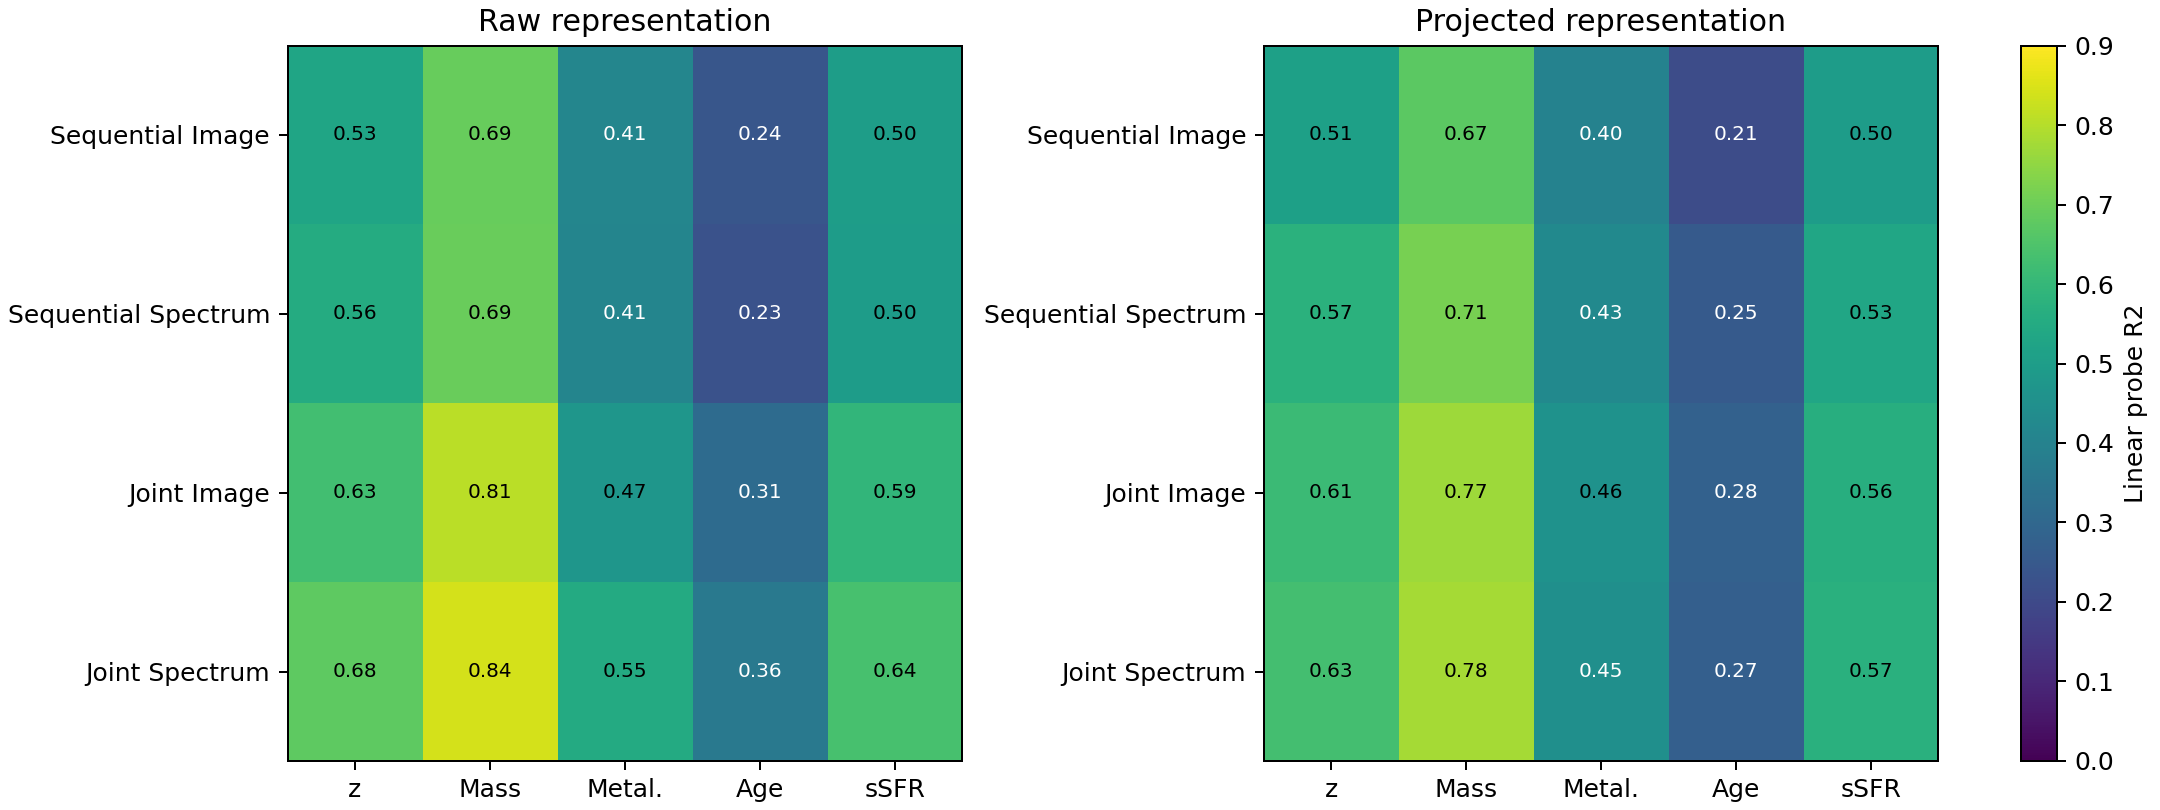
\includegraphics[width=\linewidth]{Figures/sequential/01_downstream_information.png}
\end{minipage}
\begin{minipage}{0.49\linewidth}
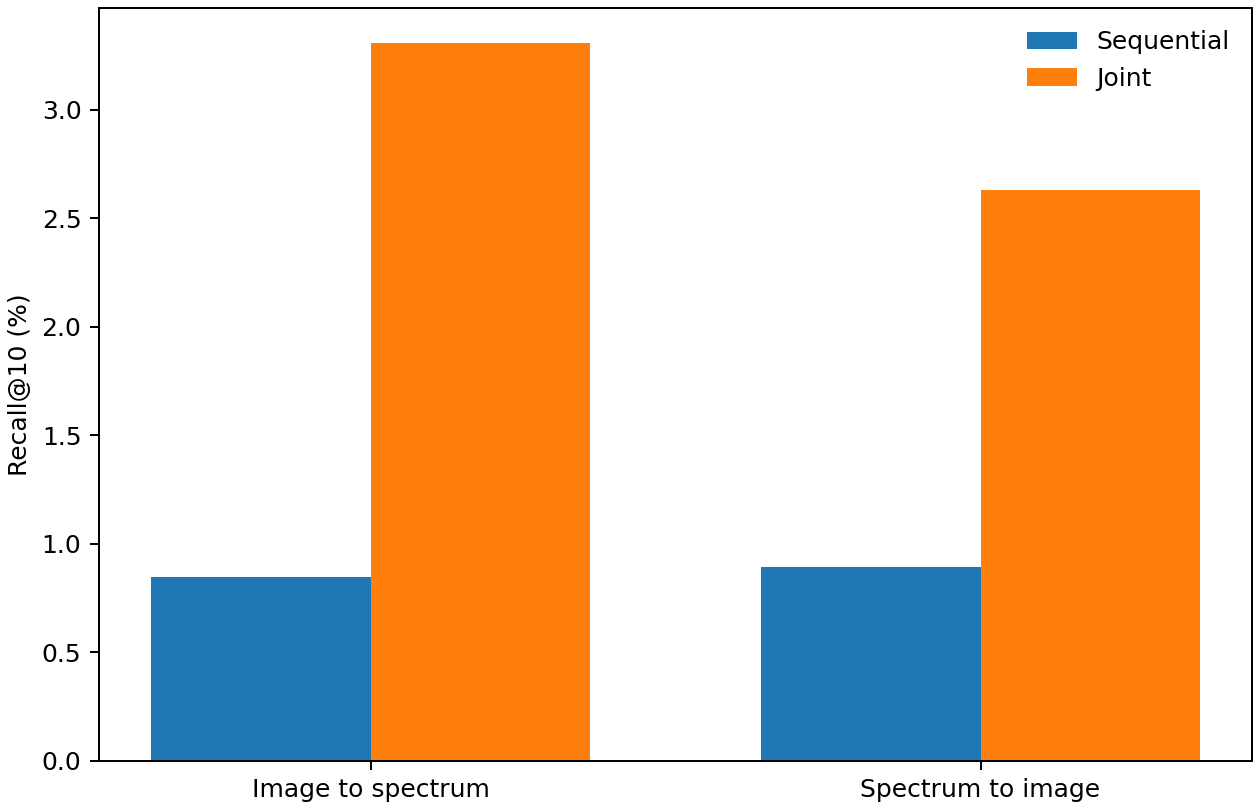
\includegraphics[width=\linewidth]{Figures/sequential/02_pair_retrieval.png}
\end{minipage}
\begin{minipage}{0.49\linewidth}
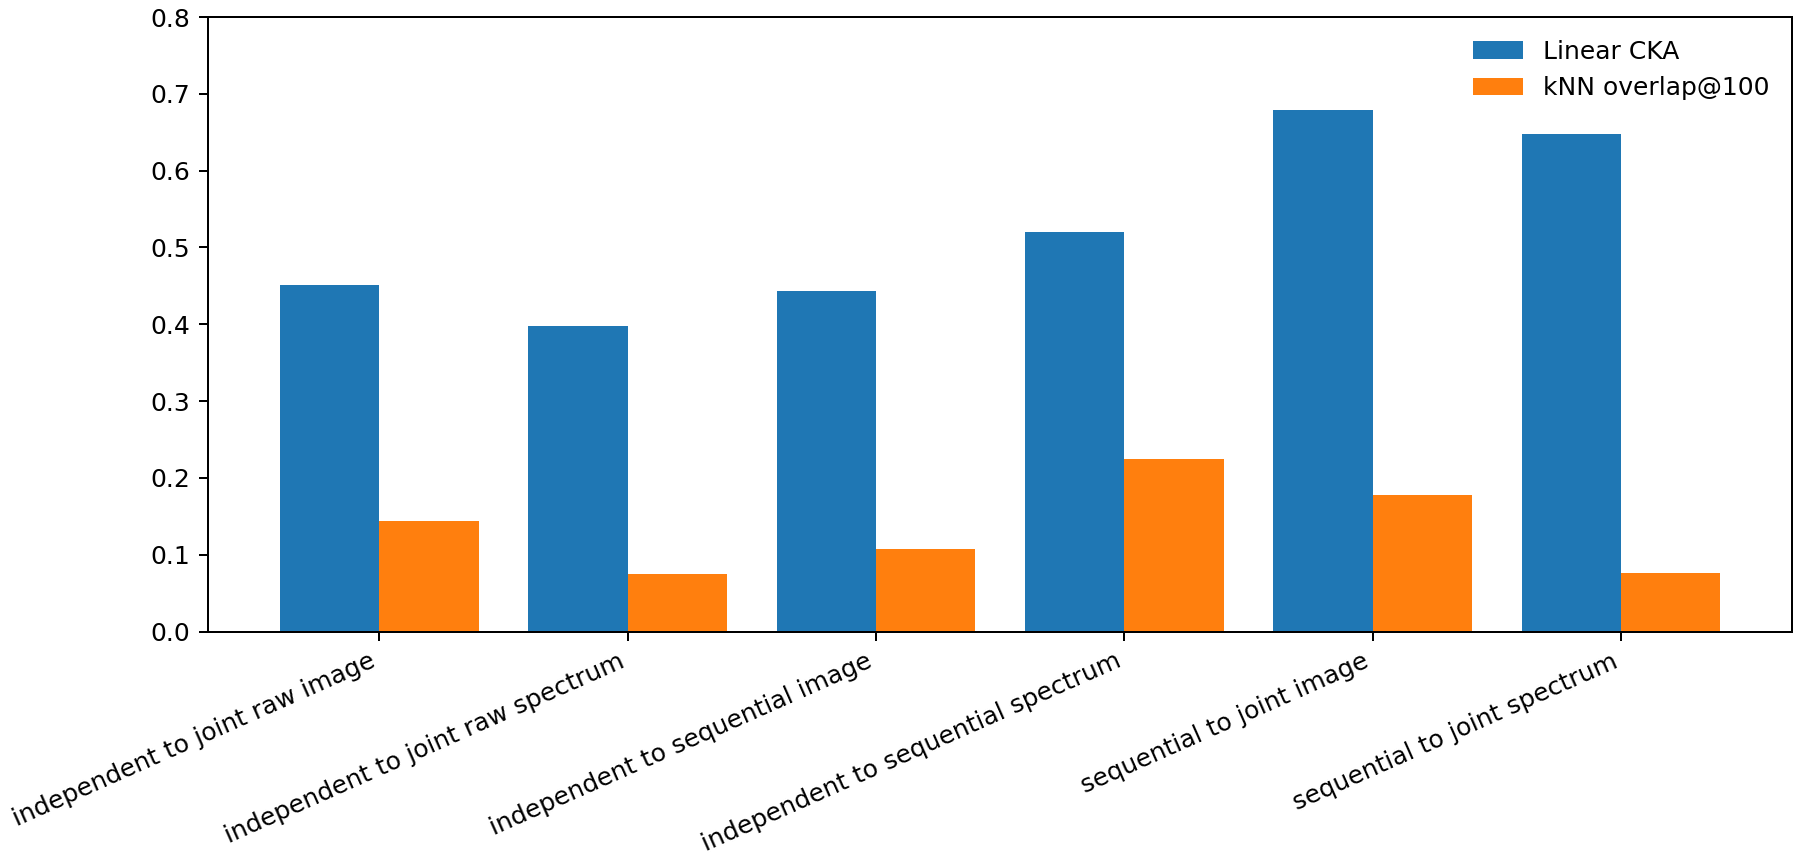
\includegraphics[width=\linewidth]{Figures/sequential/03_representation_retention.png}
\end{minipage}
\begin{minipage}{0.49\linewidth}
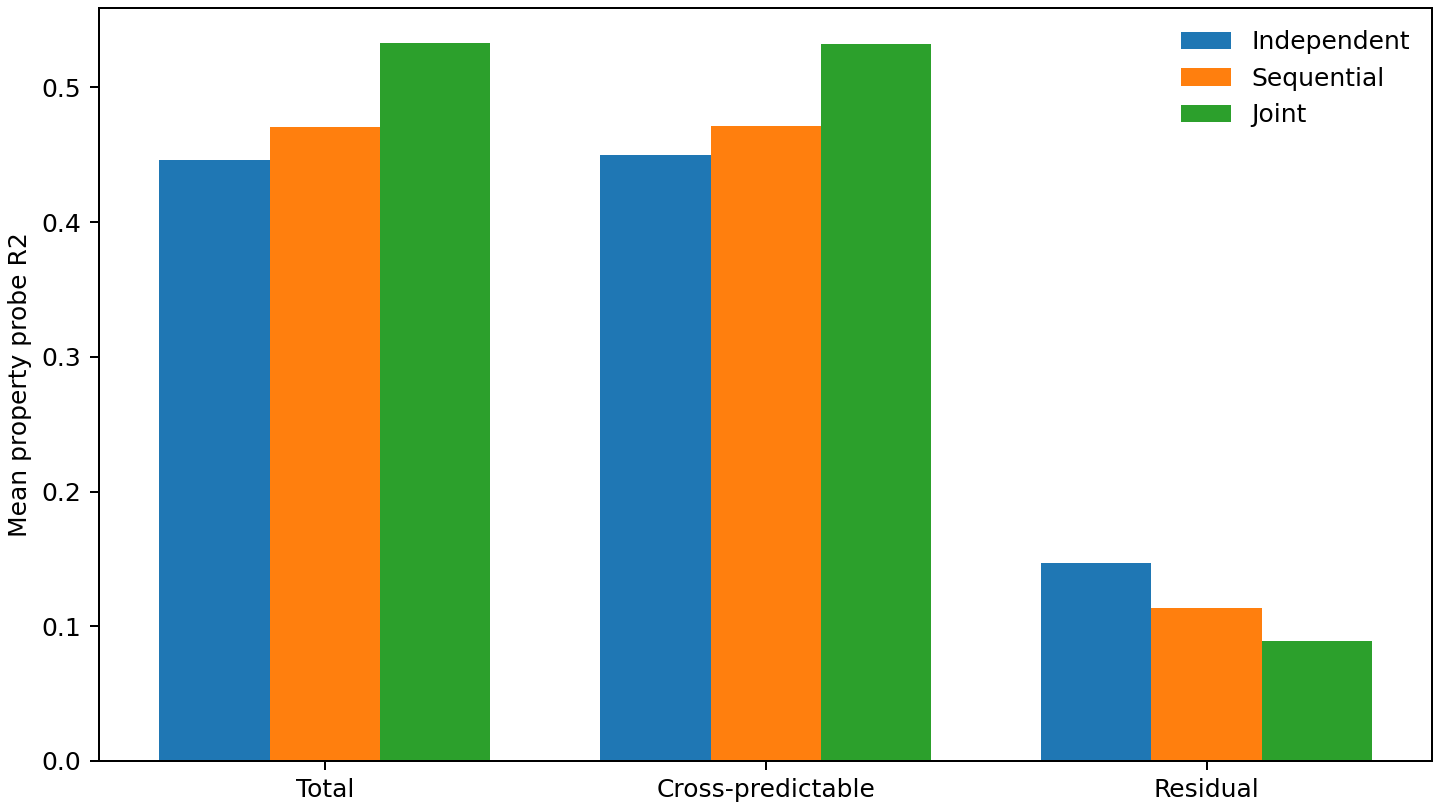
\includegraphics[width=\linewidth]{Figures/sequential/04_shared_private_accessibility.png}
\end{minipage}
\caption{The complete strategy-comparison figure set: downstream accessibility,
exact pair retrieval, representation retention, and shared/private
accessibility. Numeric values appear in
Tables~\ref{tab:full_strategy_probes}--\ref{tab:retention}.}
\label{fig:strategy_supp}
\end{figure}

\FloatBarrier
\section{Representation Analysis Before and After Alignment}
\label{app:representation}

\subsection{Raw representation retention}

\begin{table}[h]
\centering
\caption{Same-modality retention between independently pretrained, sequential,
and joint raw states. Spearman is sampled pairwise-cosine correlation.}
\label{tab:retention}
\scriptsize
\setlength{\tabcolsep}{3.5pt}
\begin{tabular}{llccccc}
\toprule
Comparison & Modality & CKA & Spearman & $k$NN@10 & $k$NN@50 & $k$NN@100\\
\midrule
Independent$\rightarrow$Joint & Image & .451 & .347 & 8.42\% & 12.18\% & 14.33\%\\
& Spectrum & .398 & .280 & 2.26\% & 5.30\% & 7.50\%\\
Independent$\rightarrow$Sequential & Image & .443 & .356 & 5.17\% & 8.47\% & 10.78\%\\
& Spectrum & .520 & .503 & 12.60\% & 18.94\% & 22.46\%\\
Sequential$\rightarrow$Joint & Image & .678 & .433 & 4.09\% & 11.68\% & 17.76\%\\
& Spectrum & .648 & .459 & 1.57\% & 4.73\% & 7.63\%\\
\bottomrule
\end{tabular}
\end{table}

The sequential raw tensors are exactly the independent backbones, but the
sequential aligned pooler summarizes token sequences rather than simply using
the standalone CLS vector.
For that reason, comparisons involving sequential outputs are not identities
even though the source backbone weights are frozen.

\subsection{Linear shared/private accessibility}

For a target state $Y$ and the opposite modality $X$, fit a train-only ridge
map $\widehat Y=A X$.
We call $\widehat Y$ shared and $Y-\widehat Y$ private, then fit the same
scientific probes separately.
The construction is operational: it does not estimate mutual information or
guarantee statistical independence.

\begin{table}[h]
\centering
\caption{Mean \rscore\ across redshift, mass, metallicity, age, and sSFR for
total, cross-modally predictable, and residual components. Map is the
global held-out cross-modal \rscore.}
\label{tab:shared_private}
\small
\begin{tabular}{llrrrr}
\toprule
State & Predicted target & Total & Shared & Residual & Map\\
\midrule
Independent & Spectrum & .455 & .440 & .156 & .025\\
& Image & .438 & .459 & .138 & .025\\
\prealign & Spectrum & .493 & .452 & .152 & .597\\
& Image & .449 & .491 & .075 & .626\\
\joint & Spectrum & .535 & .531 & .107 & .749\\
& Image & .531 & .534 & .071 & .736\\
\bottomrule
\end{tabular}
\end{table}

Shared-component scores can slightly exceed total scores because the learned
cross-modal map suppresses probe-irrelevant variation.
Residual scores need not vanish because nonlinear shared signal, finite-sample
mapping error, and modality-private information are all present.

\subsection{Morphology retention}

\begin{table}[h]
\centering
\caption{Galaxy10 morphology retained by image states.}
\label{tab:morphology_retention}
\small
\begin{tabular}{lcc}
\toprule
Image state & Accuracy (\%) & Macro-F1 (\%)\\
\midrule
Independent raw & $71.83\pm0.84$ & $70.23\pm0.90$\\
\prealign\ shared & $59.63\pm1.20$ & $57.53\pm1.14$\\
\joint\ raw & $72.22\pm1.26$ & $70.19\pm1.30$\\
\joint\ shared & $44.99\pm0.97$ & $42.77\pm0.97$\\
\bottomrule
\end{tabular}
\end{table}

\begin{figure}[h]
\centering
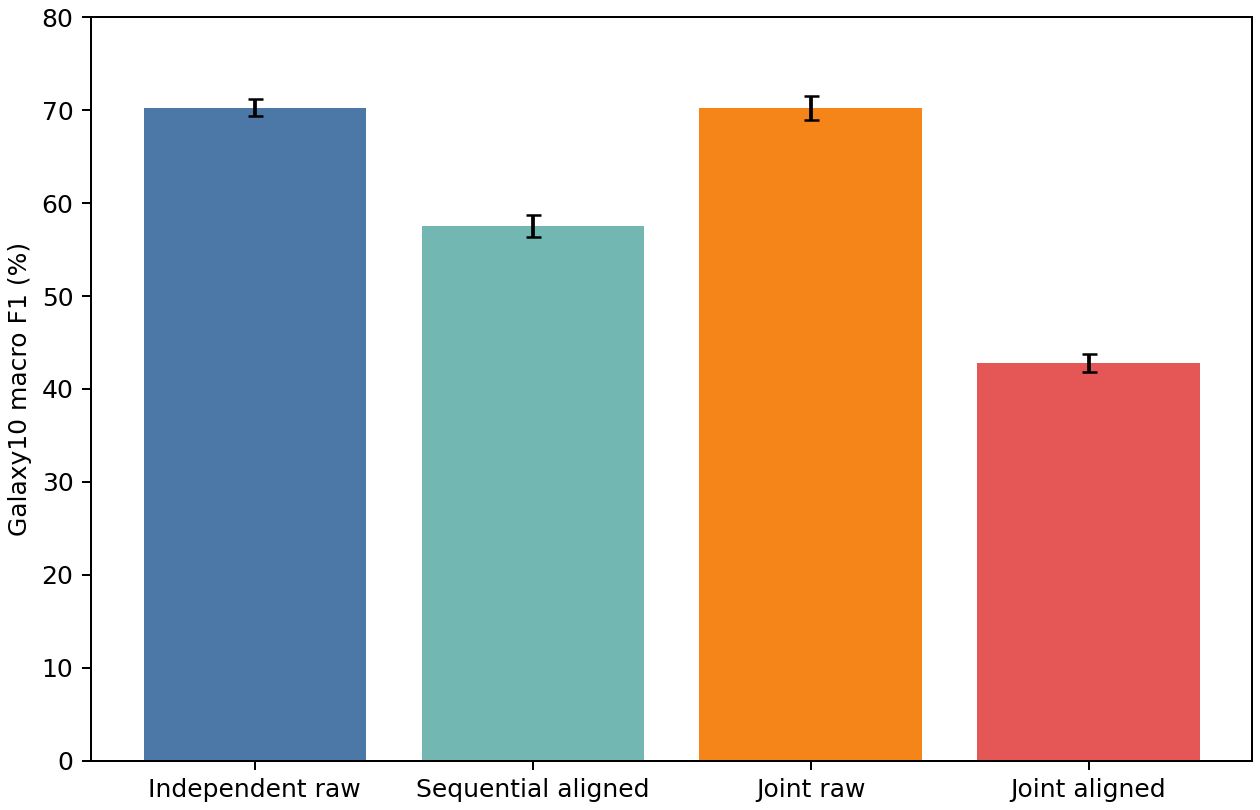
\includegraphics[width=.72\linewidth]{Figures/sequential/05_morphology_retention.png}
\caption{The joint raw backbone preserves morphology while the shared
projection filters it. Error bars are standard deviations across three
stratified Galaxy10 splits.}
\label{fig:morphology_retention}
\end{figure}

\FloatBarrier
\section{Contrastive Baselines: Detailed JEPA vs.\ CLIP}
\label{app:clip}

\subsection{Frozen-backbone objective ablation}

Before the end-to-end comparison, we aligned the same frozen unimodal
backbones with two learned-query adapter systems.
The JEPA+SIGReg adapter has 256-dimensional output and 2.23M trainable
parameters; the released-code-style InfoNCE adapter has 512-dimensional output
and 7.09M trainable parameters.
Both use the same 307,428 pairs for 10 epochs, but JEPA+SIGReg uses global
batch 128 for 24,000 updates and InfoNCE uses global batch 256 for 12,000.
The objective, dimensionality, parameter count, and update granularity are
therefore jointly varied.

\begin{table}[h]
\centering
\caption{Frozen-adapter objective ablation, with the two end-to-end runs shown
for context. Values are shared-space probe \rscore.}
\label{tab:frozen_infonce}
\small
\setlength{\tabcolsep}{4.0pt}
\begin{tabular}{lrrrr}
\toprule
Target & Post JEPA & Post InfoNCE & Scratch JEPA & Scratch CLIP\\
\midrule
Image redshift & .5118 & .5417 & \textbf{.6137} & .6016\\
Spectrum redshift & .5739 & .5868 & .6322 & \textbf{.6515}\\
Stellar mass & .7176 & .7482 & .7815 & \textbf{.8169}\\
sSFR & .5330 & .5664 & .5701 & \textbf{.6279}\\
Metallicity & .4282 & .4424 & .4482 & \textbf{.5089}\\
Stellar age & .2584 & .2643 & .2758 & \textbf{.3555}\\
\bottomrule
\end{tabular}
\end{table}

InfoNCE improves every tested frozen-adapter target.
Its image/spectrum effective ranks are 12.01/12.85 in 512 dimensions, versus
8.83/8.60 in 256 dimensions for JEPA+SIGReg; the unequal dimensions prevent a
strict rank comparison.
Both end-to-end systems outperform both frozen adapters on every row.
This supports paired backbone adaptation, while leaving open whether
fine-tuned unimodal initialization would outperform random initialization.

\subsection{Control boundary}

The scratch JEPA+SIGReg and CLIP runs use identical randomly initialized
architectures, paired objects, view generators, and 50-epoch sample exposure.
JEPA+SIGReg uses global batch 256 and 60,000 updates; CLIP uses global batch 128,
127 in-batch negatives per anchor, and 120,000 updates.
Thus the comparison is architecture- and sample-matched but partially confounds
objective, batch, and optimizer granularity.

\begin{table}[h]
\centering
\caption{Exact test-pool retrieval. Recall is percent.}
\label{tab:clip_retrieval}
\small
\begin{tabular}{llrrrrr}
\toprule
Objective & Direction & R@1 & R@5 & R@10 & Median rank & MRR\\
\midrule
JEPA+SIGReg & I$\rightarrow$S & .461 & 1.805 & 3.307 & 429 & .01786\\
& S$\rightarrow$I & .320 & 1.431 & 2.633 & 454 & .01475\\
CLIP & I$\rightarrow$S & \textbf{1.488} & \textbf{5.378} & \textbf{8.772} & \textbf{230} & \textbf{.04235}\\
& S$\rightarrow$I & \textbf{1.054} & \textbf{4.152} & \textbf{7.193} & \textbf{270} & \textbf{.03449}\\
\bottomrule
\end{tabular}
\end{table}

\begin{table}[h]
\centering
\caption{Global, local, and information alignment. Neighborhood values are the
machine-readable CSV results; they supersede rounded draft-report values.}
\label{tab:clip_geometry}
\small
\setlength{\tabcolsep}{4.5pt}
\begin{tabular}{lcc}
\toprule
Metric & JEPA+SIGReg & CLIP\\
\midrule
Projected cross-modal CKA & \textbf{.7705} & .6338\\
Raw cross-modal CKA & \textbf{.8983} & .8320\\
Pairwise-geometry Spearman & \textbf{.6073} & .4845\\
$k$NN overlap@10 & 1.702\% & \textbf{2.621\%}\\
$k$NN overlap@50 & 6.263\% & \textbf{7.256\%}\\
$k$NN overlap@100 & 10.488\% & \textbf{10.969\%}\\
Map I$\rightarrow$S \rscore & \textbf{.7492} & .5507\\
Map S$\rightarrow$I \rscore & \textbf{.7365} & .5491\\
CCA top 10 & \textbf{.9156} & .9046\\
CCA top 50 & \textbf{.6750} & .6579\\
CCA all dimensions & .2118 & \textbf{.2156}\\
\bottomrule
\end{tabular}
\end{table}

\FloatBarrier
The two metric families are not contradictory.
Exact retrieval is a tail-ranking statistic, whereas CKA, sampled distance
correlation, and map \rscore\ summarize many global relations.
CLIP's negatives directly train competitive instance ranking; SIGReg-supported
invariance produces a more linearly transformable manifold.

\subsection{Scientific probes and dimensional use}

\begin{table}[h]
\centering
\caption{All raw and projected probe \rscore\ for the scratch objective
comparison. Bold marks the stronger objective within each modality/state.}
\label{tab:clip_probes}
\scriptsize
\setlength{\tabcolsep}{3.5pt}
\begin{tabular}{lllccccc}
\toprule
Objective & Modality & State & Redshift & Mass & Metal. & Age & sSFR\\
\midrule
\multirow{4}{*}{JEPA+SIGReg}
& Image & raw & \textbf{.627} & \textbf{.806} & \textbf{.474} & \textbf{.314} & \textbf{.591}\\
& Image & shared & \textbf{.613} & .768 & .459 & .278 & .564\\
& Spectrum & raw & .675 & .842 & .549 & .363 & .639\\
& Spectrum & shared & .632 & .780 & .448 & .274 & .570\\
\midrule
\multirow{4}{*}{CLIP}
& Image & raw & .610 & .793 & .465 & .307 & .580\\
& Image & shared & .601 & \textbf{.792} & \textbf{.469} & \textbf{.306} & \textbf{.583}\\
& Spectrum & raw & \textbf{.678} & \textbf{.846} & \textbf{.567} & \textbf{.391} & \textbf{.663}\\
& Spectrum & shared & \textbf{.651} & \textbf{.816} & \textbf{.509} & \textbf{.353} & \textbf{.628}\\
\bottomrule
\end{tabular}
\end{table}

\begin{table}[h]
\centering
\caption{Effective rank. CLIP distributes variance over more directions, while
JEPA+SIGReg yields stronger global cross-modal congruence.}
\label{tab:clip_rank}
\small
\begin{tabular}{lrrrr}
\toprule
Objective & Image raw & Spectrum raw & Image shared & Spectrum shared\\
\midrule
JEPA+SIGReg & 28.26 & 26.08 & 20.19 & 17.94\\
CLIP & \textbf{64.29} & \textbf{58.14} & \textbf{45.39} & \textbf{44.65}\\
\bottomrule
\end{tabular}
\end{table}

\FloatBarrier
Same-modality CKA between objectives is 0.9395 for raw image states and 0.8528
for raw spectra.
The backbones therefore remain broadly related even though the shared heads and
cross-modal behavior differ.

\subsection{Linear alignment and decoder transfer}

After per-modality train-set standardization, an orthogonal Procrustes map
modestly improves exact retrieval:
JEPA+SIGReg I$\rightarrow$S R@1 rises from 0.44\% to 0.54\% and
S$\rightarrow$I from 0.30\% to 0.45\%;
CLIP rises from 1.55\% to 2.02\% and 1.49\% to 1.84\%, respectively.
Matched cosine similarity changes from 0.780 to 0.806 for JEPA+SIGReg and from
0.402 to 0.595 for CLIP.
These standardized before-values are not the raw-cosine baselines in
Table~\ref{tab:clip_retrieval}.
The limited retrieval recovery despite high CCA implies more than a simple
rotation separates the modalities.

\begin{table}[h]
\centering
\caption{Probe-decoder transfer after Procrustes alignment. Each decoder is
trained on the source named in the direction and evaluated on the other
modality. Values are \rscore.}
\label{tab:decoder_transfer}
\scriptsize
\setlength{\tabcolsep}{3.6pt}
\begin{tabular}{llccccc}
\toprule
Objective & Decoder transfer & Redshift & Mass & Metal. & Age & sSFR\\
\midrule
JEPA+SIGReg & Image decoder on spectrum & .515 & .621 & .369 & .166 & .474\\
CLIP & Image decoder on spectrum & .467 & \textbf{.626} & .355 & \textbf{.225} & .365\\
JEPA+SIGReg & Spectrum decoder on image & .529 & .630 & .373 & \textbf{.219} & .495\\
CLIP & Spectrum decoder on image & .502 & \textbf{.666} & .372 & .214 & .441\\
\bottomrule
\end{tabular}
\end{table}

\FloatBarrier
Direct decoder transfer without alignment is frequently poor or negative.
The complete own-space, direct-transfer, and Procrustes-transfer values are
visualized in Figure~\ref{fig:objective_extra} and stored with the study CSVs.

\begin{figure}[p]
\centering
\begin{minipage}{0.49\linewidth}
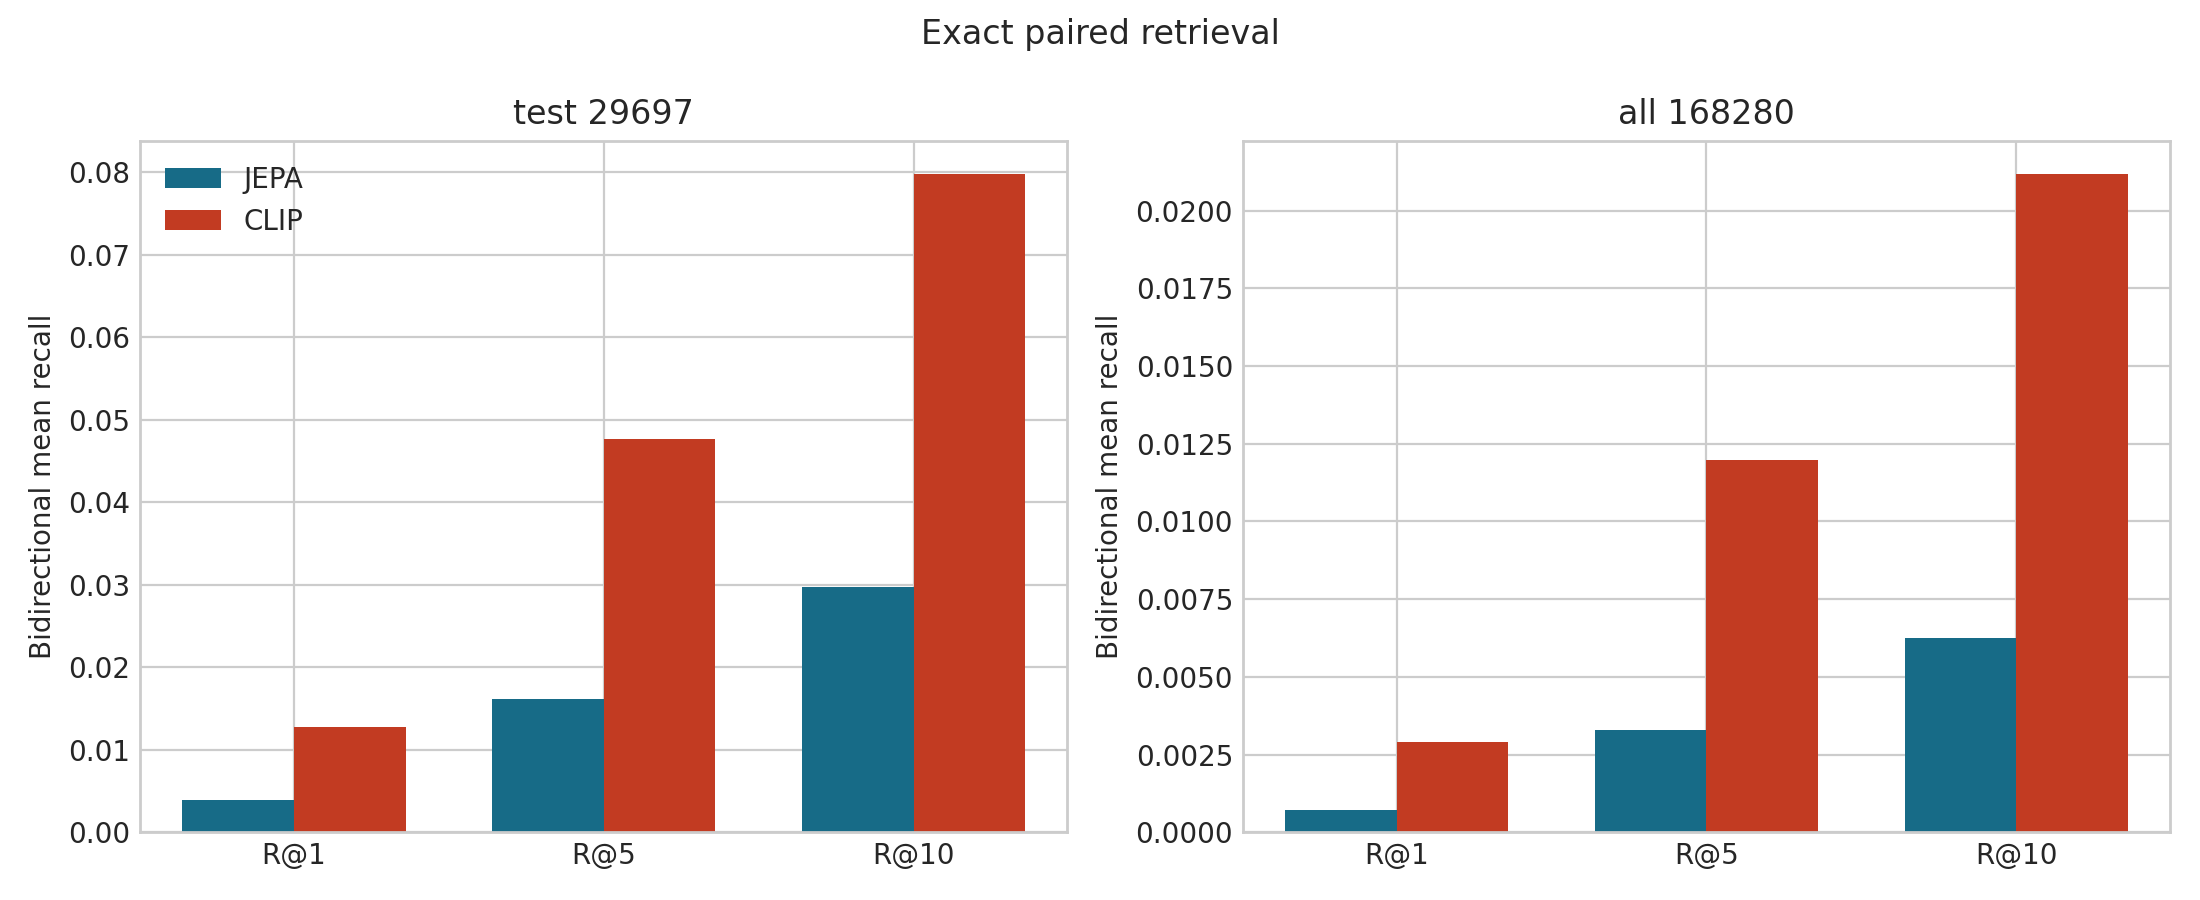
\includegraphics[width=\linewidth]{Figures/objectives/01_retrieval.png}
\end{minipage}
\begin{minipage}{0.49\linewidth}
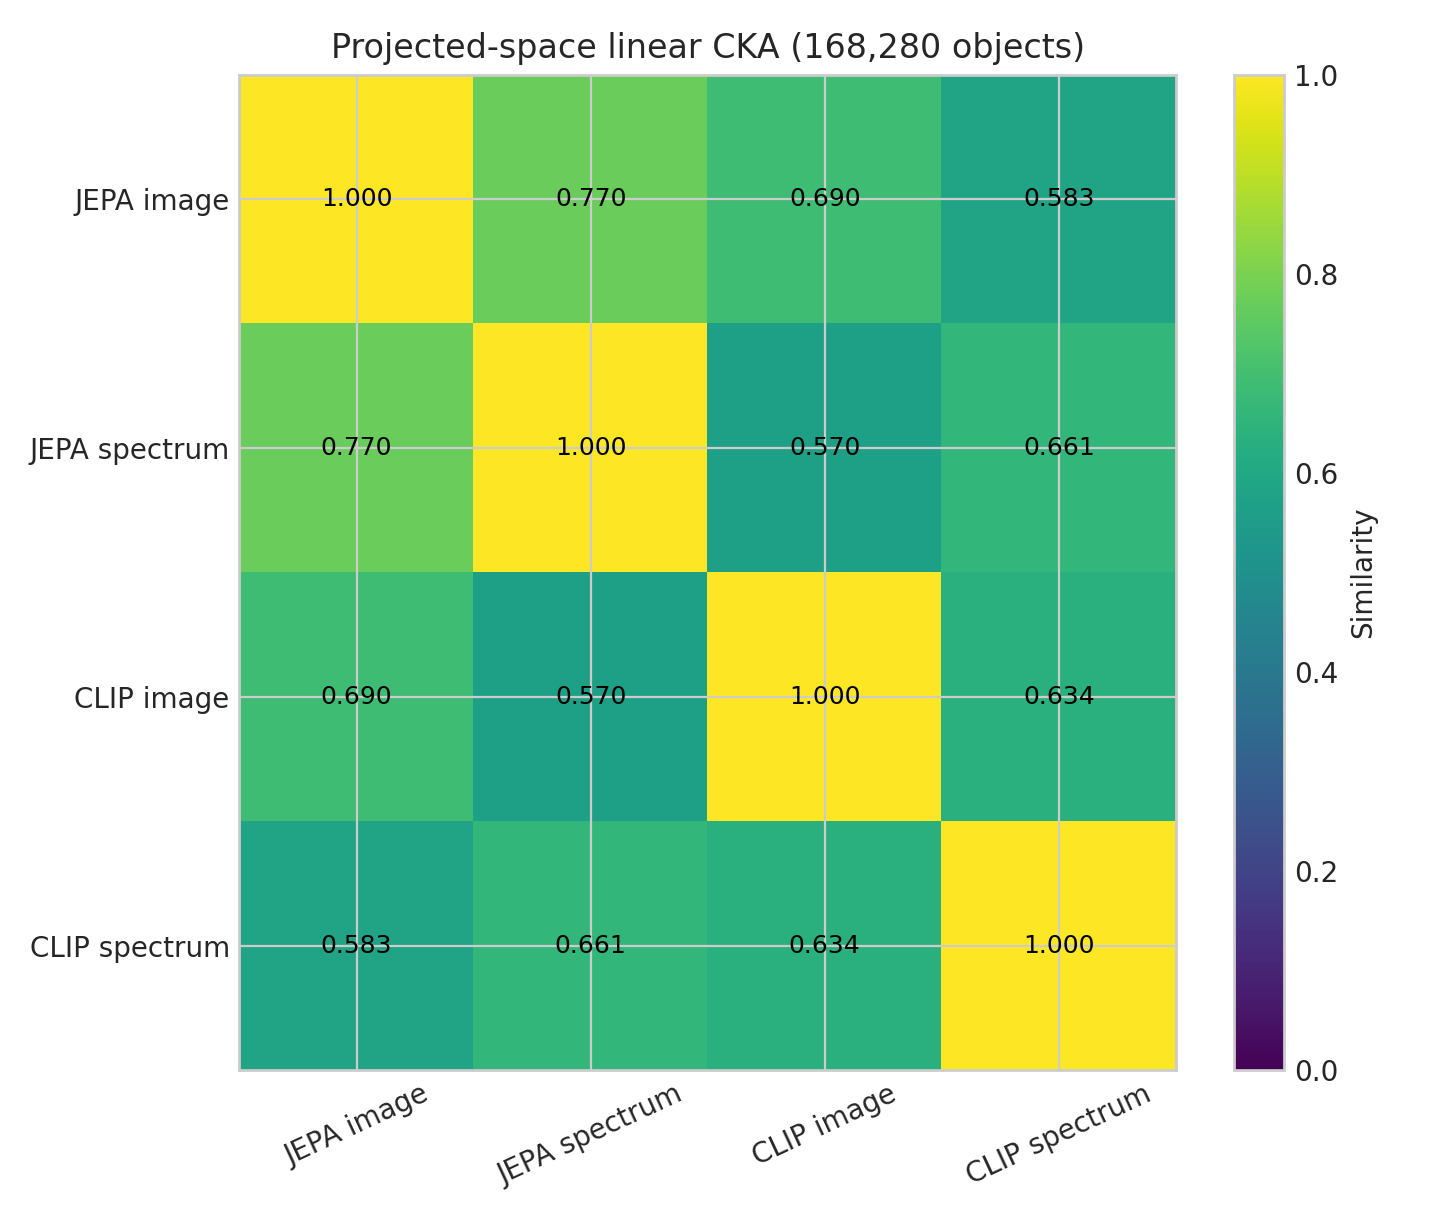
\includegraphics[width=\linewidth]{Figures/objectives/02_cka_projected.png}
\end{minipage}
\begin{minipage}{0.49\linewidth}
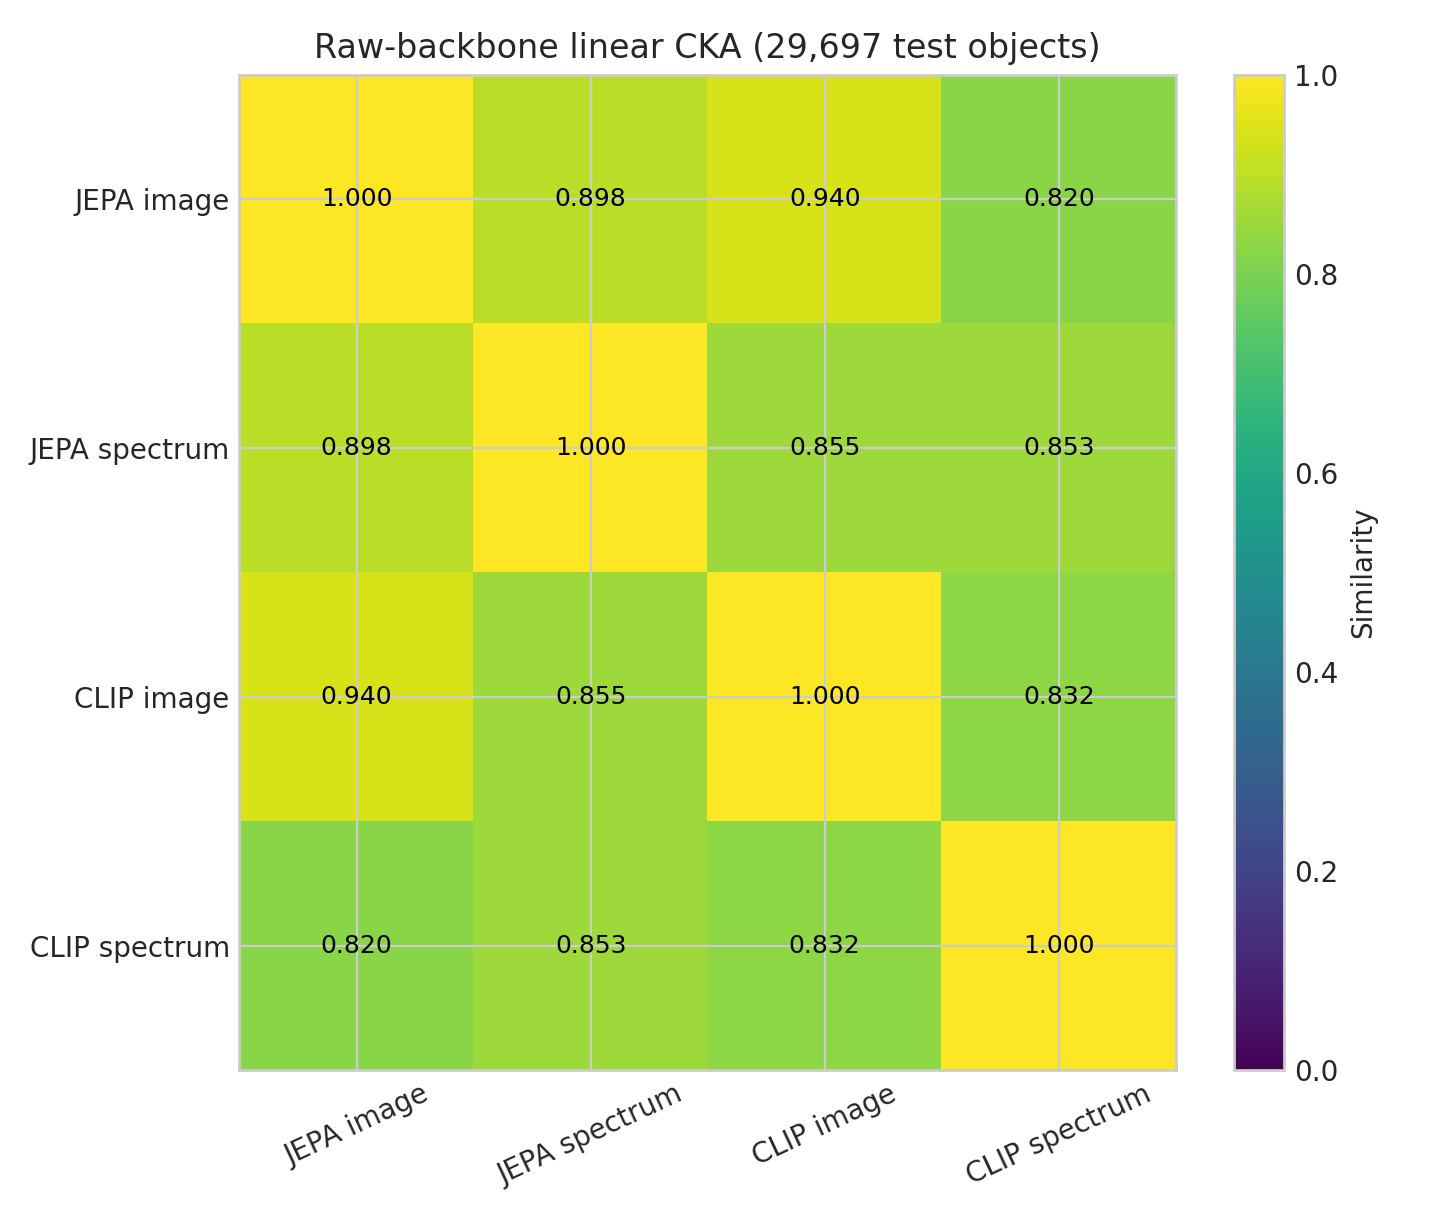
\includegraphics[width=\linewidth]{Figures/objectives/03_cka_raw.png}
\end{minipage}
\begin{minipage}{0.49\linewidth}
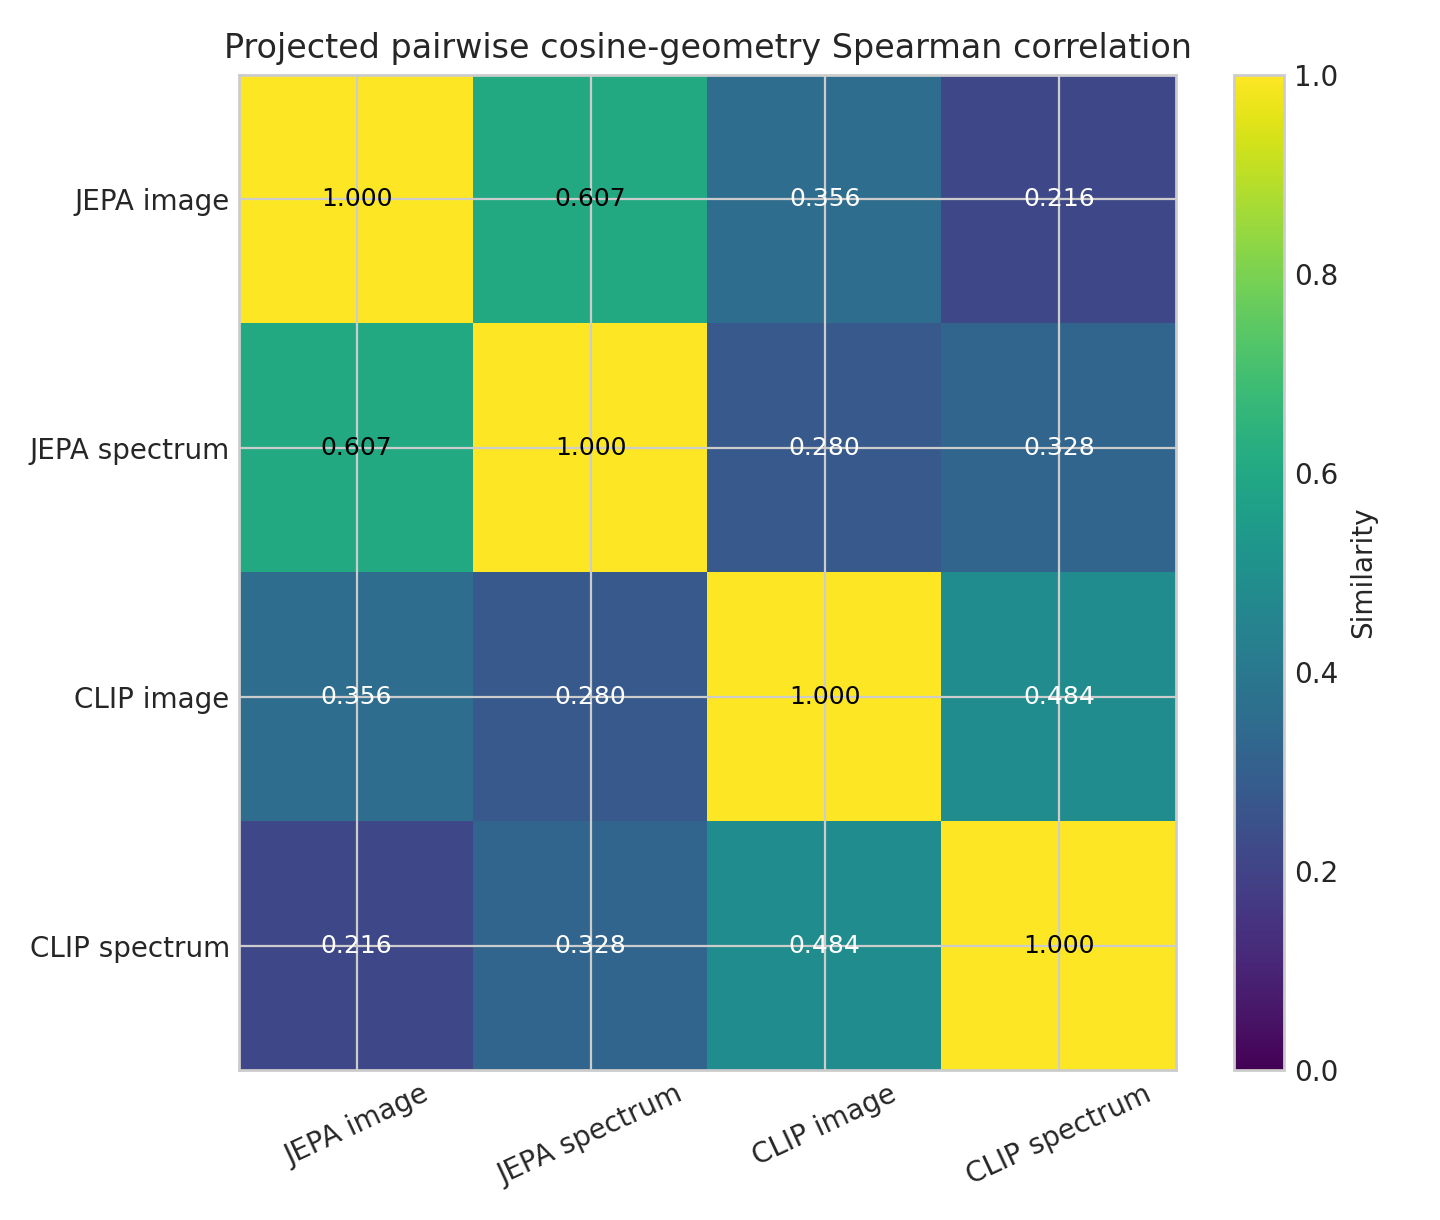
\includegraphics[width=\linewidth]{Figures/objectives/04_distance_spearman.png}
\end{minipage}
\begin{minipage}{0.49\linewidth}
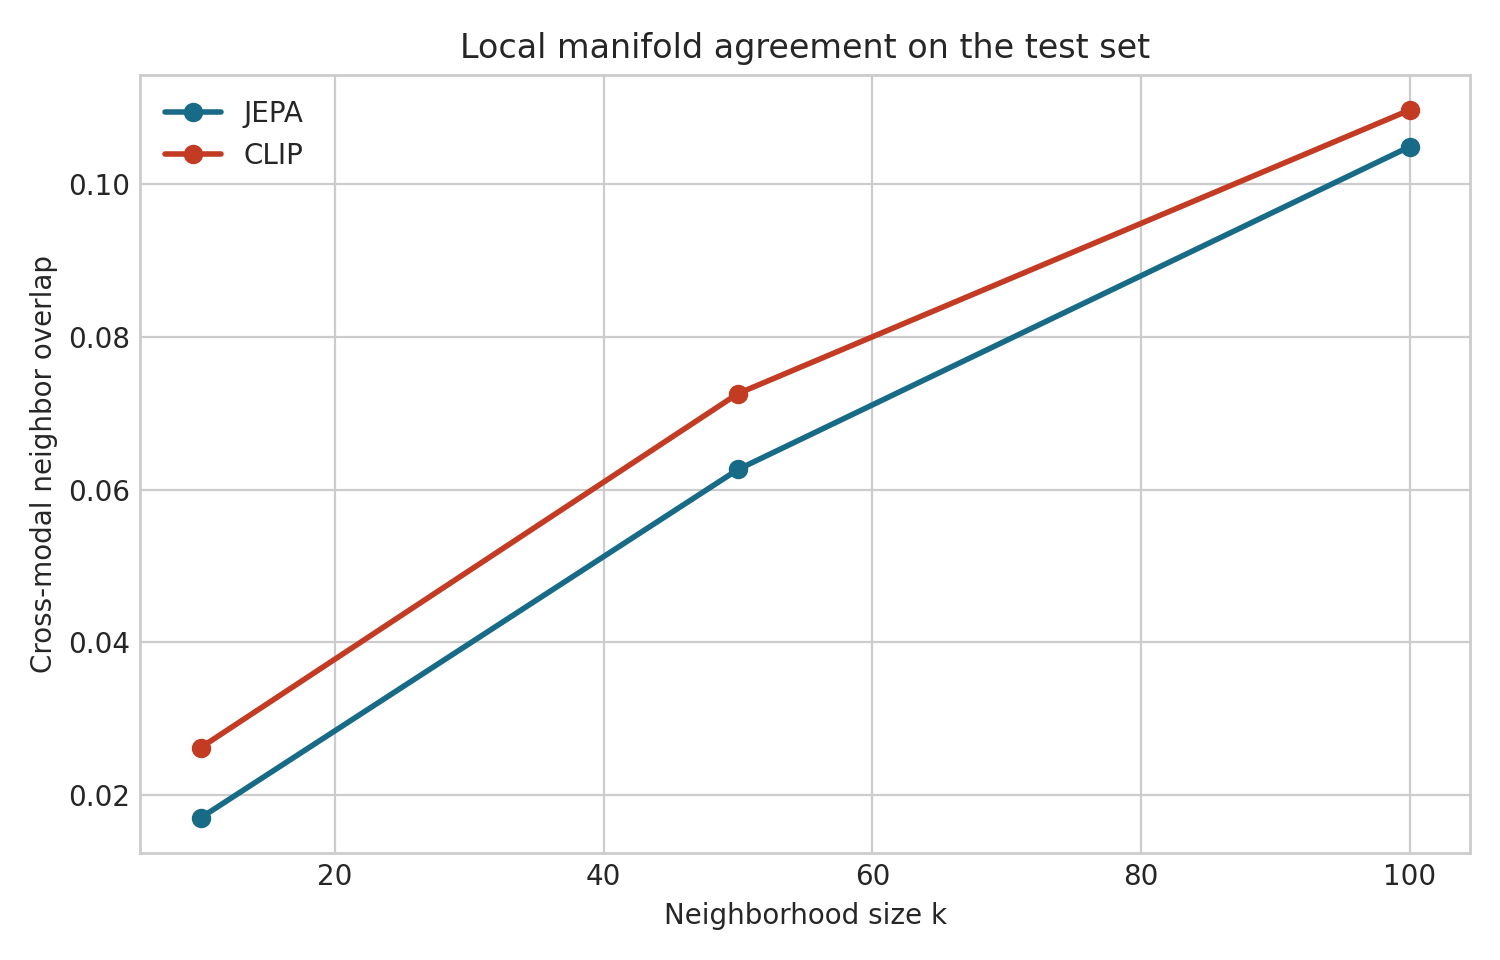
\includegraphics[width=\linewidth]{Figures/objectives/05_neighborhood_overlap.png}
\end{minipage}
\begin{minipage}{0.49\linewidth}
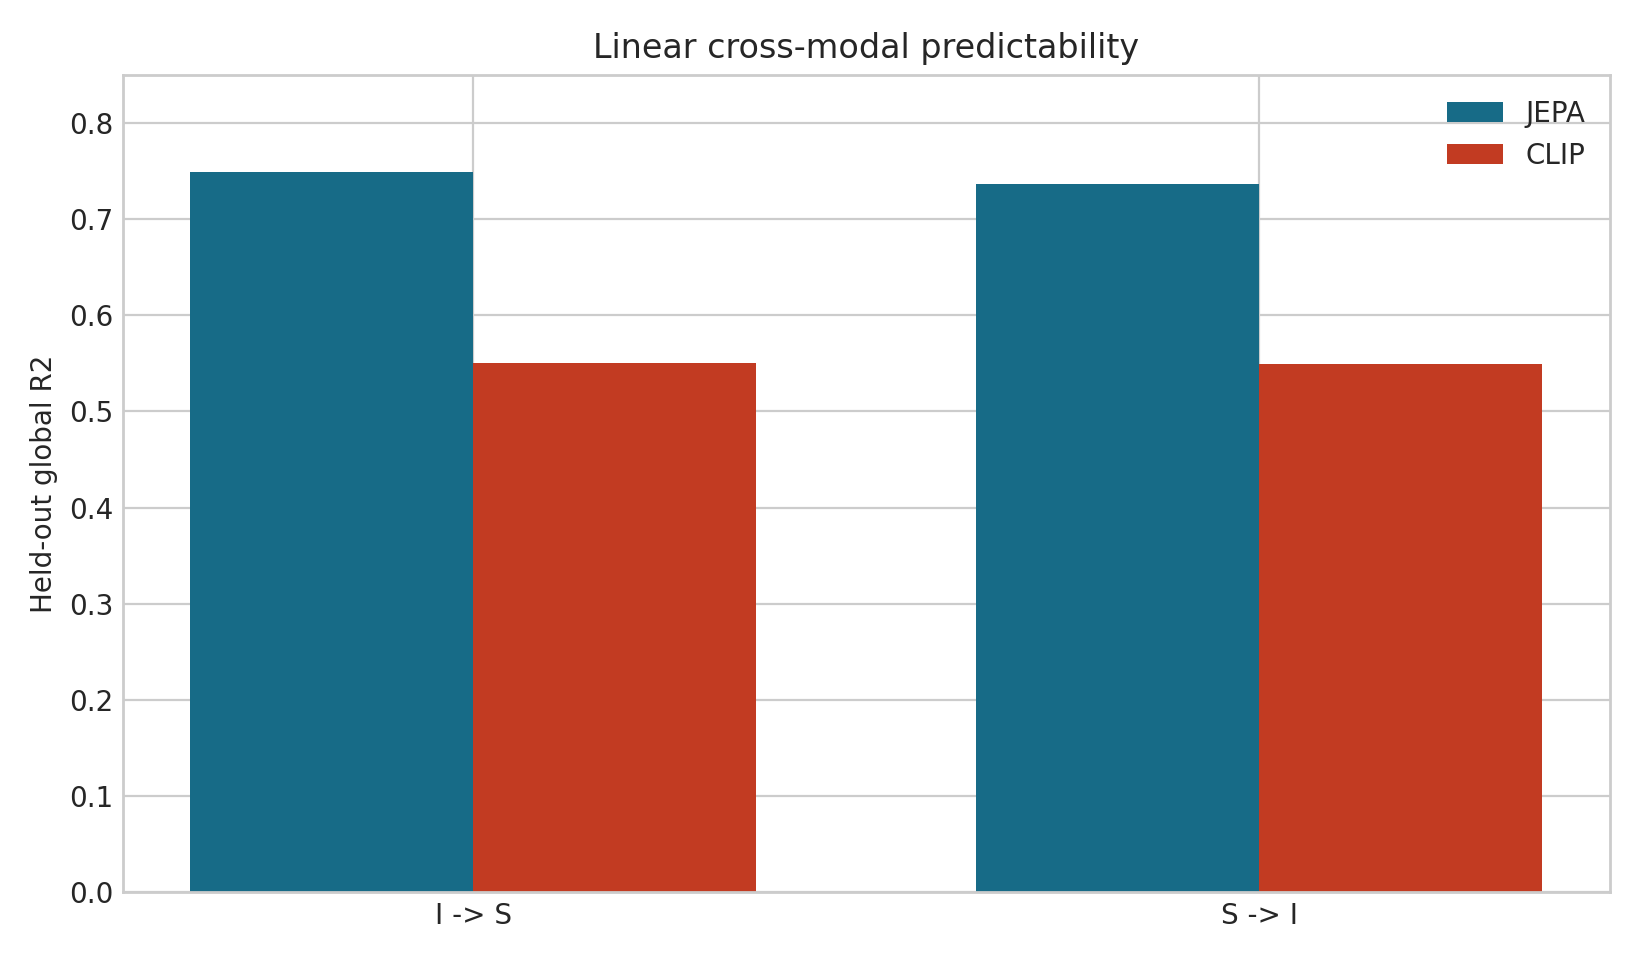
\includegraphics[width=\linewidth]{Figures/objectives/06_linear_predictability.png}
\end{minipage}
\caption{Primary JEPA+SIGReg versus CLIP diagnostics: exact retrieval, projected
and raw CKA, pairwise geometry, local-neighborhood overlap, and linear
cross-modal predictability.}
\label{fig:objective_primary}
\end{figure}

\begin{figure}[p]
\centering
\begin{minipage}{0.49\linewidth}
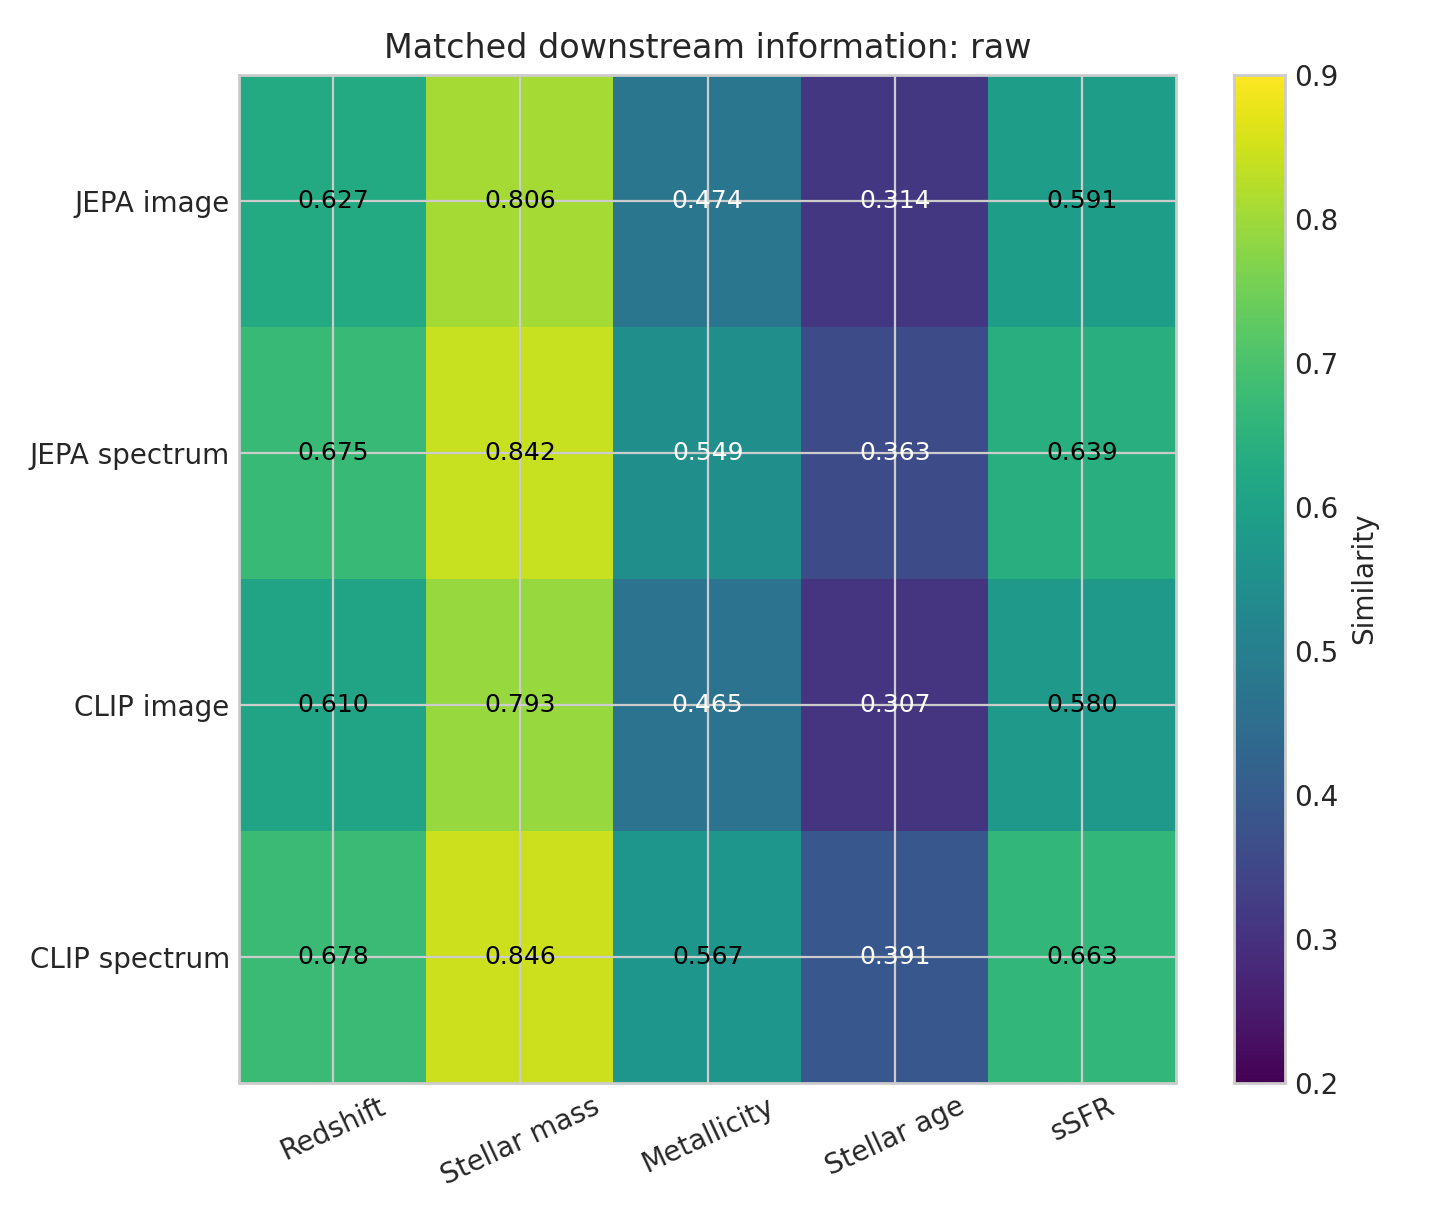
\includegraphics[width=\linewidth]{Figures/objectives/07_downstream_raw.png}
\end{minipage}
\begin{minipage}{0.49\linewidth}
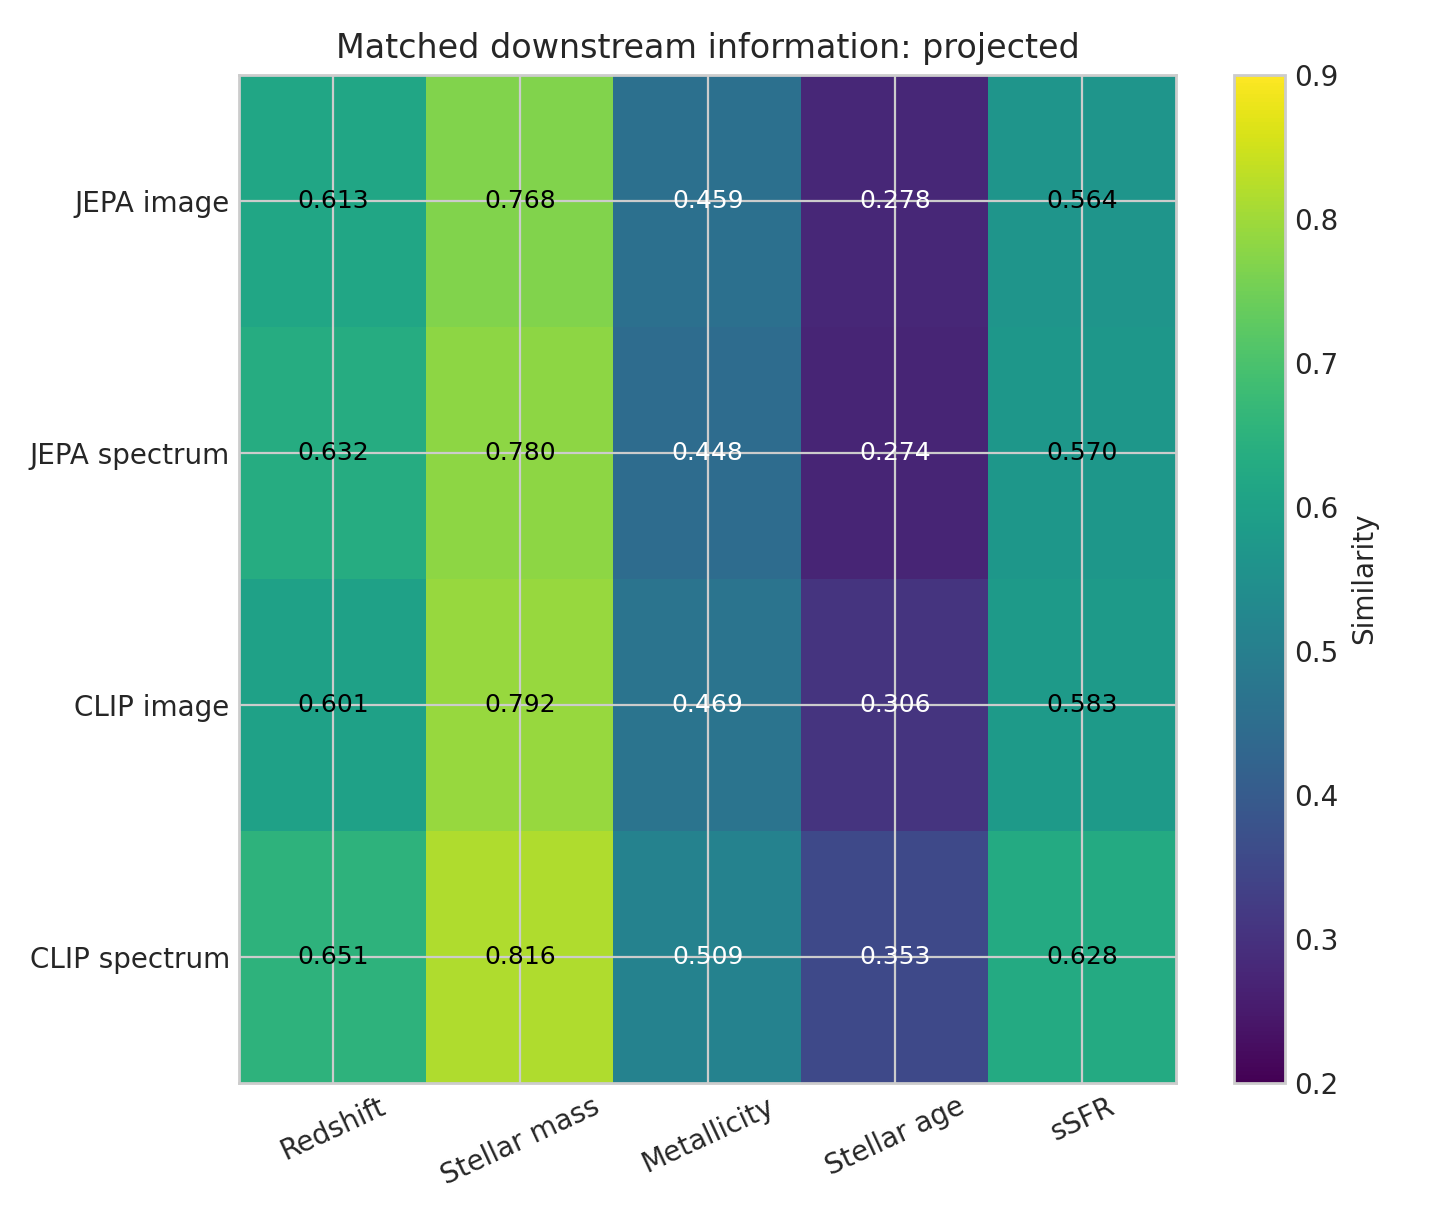
\includegraphics[width=\linewidth]{Figures/objectives/07_downstream_projected.png}
\end{minipage}
\begin{minipage}{0.49\linewidth}
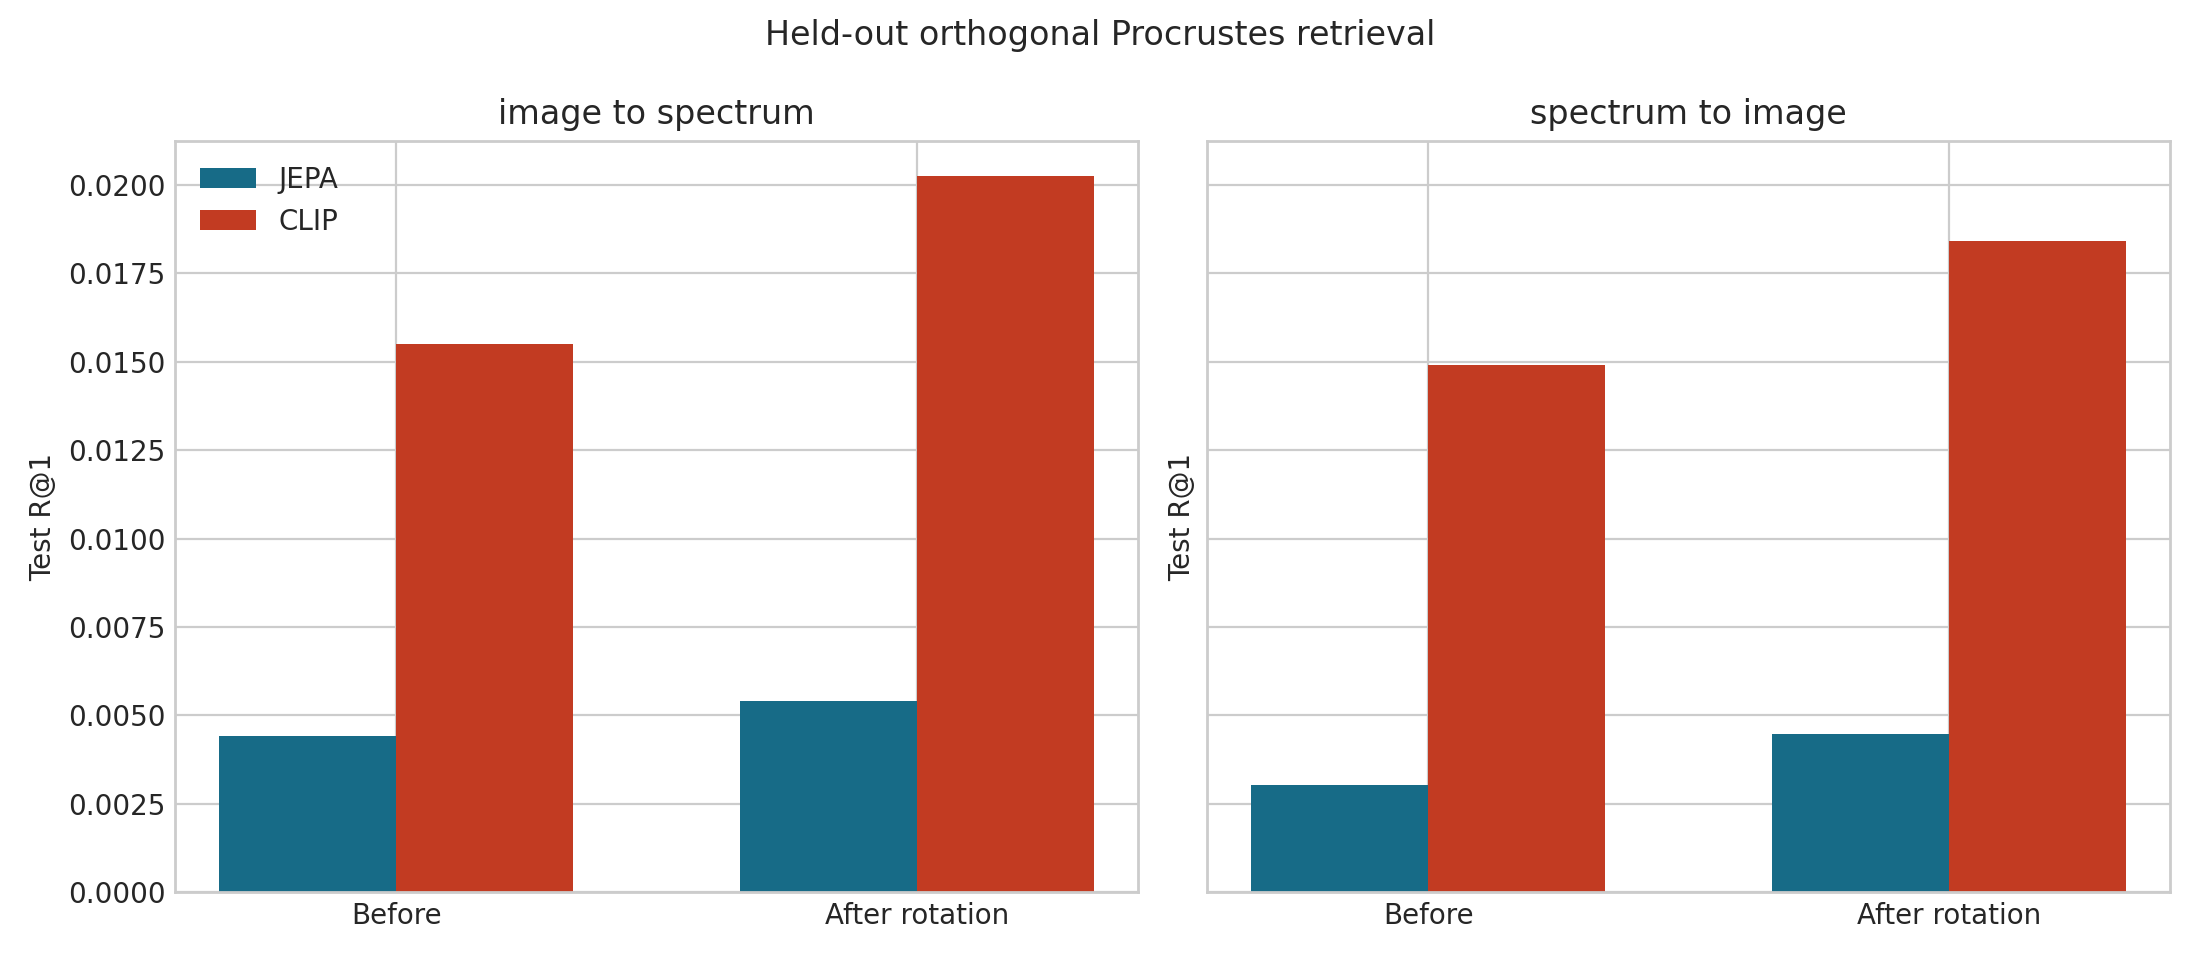
\includegraphics[width=\linewidth]{Figures/objectives/08_procrustes_retrieval.png}
\end{minipage}
\begin{minipage}{0.49\linewidth}
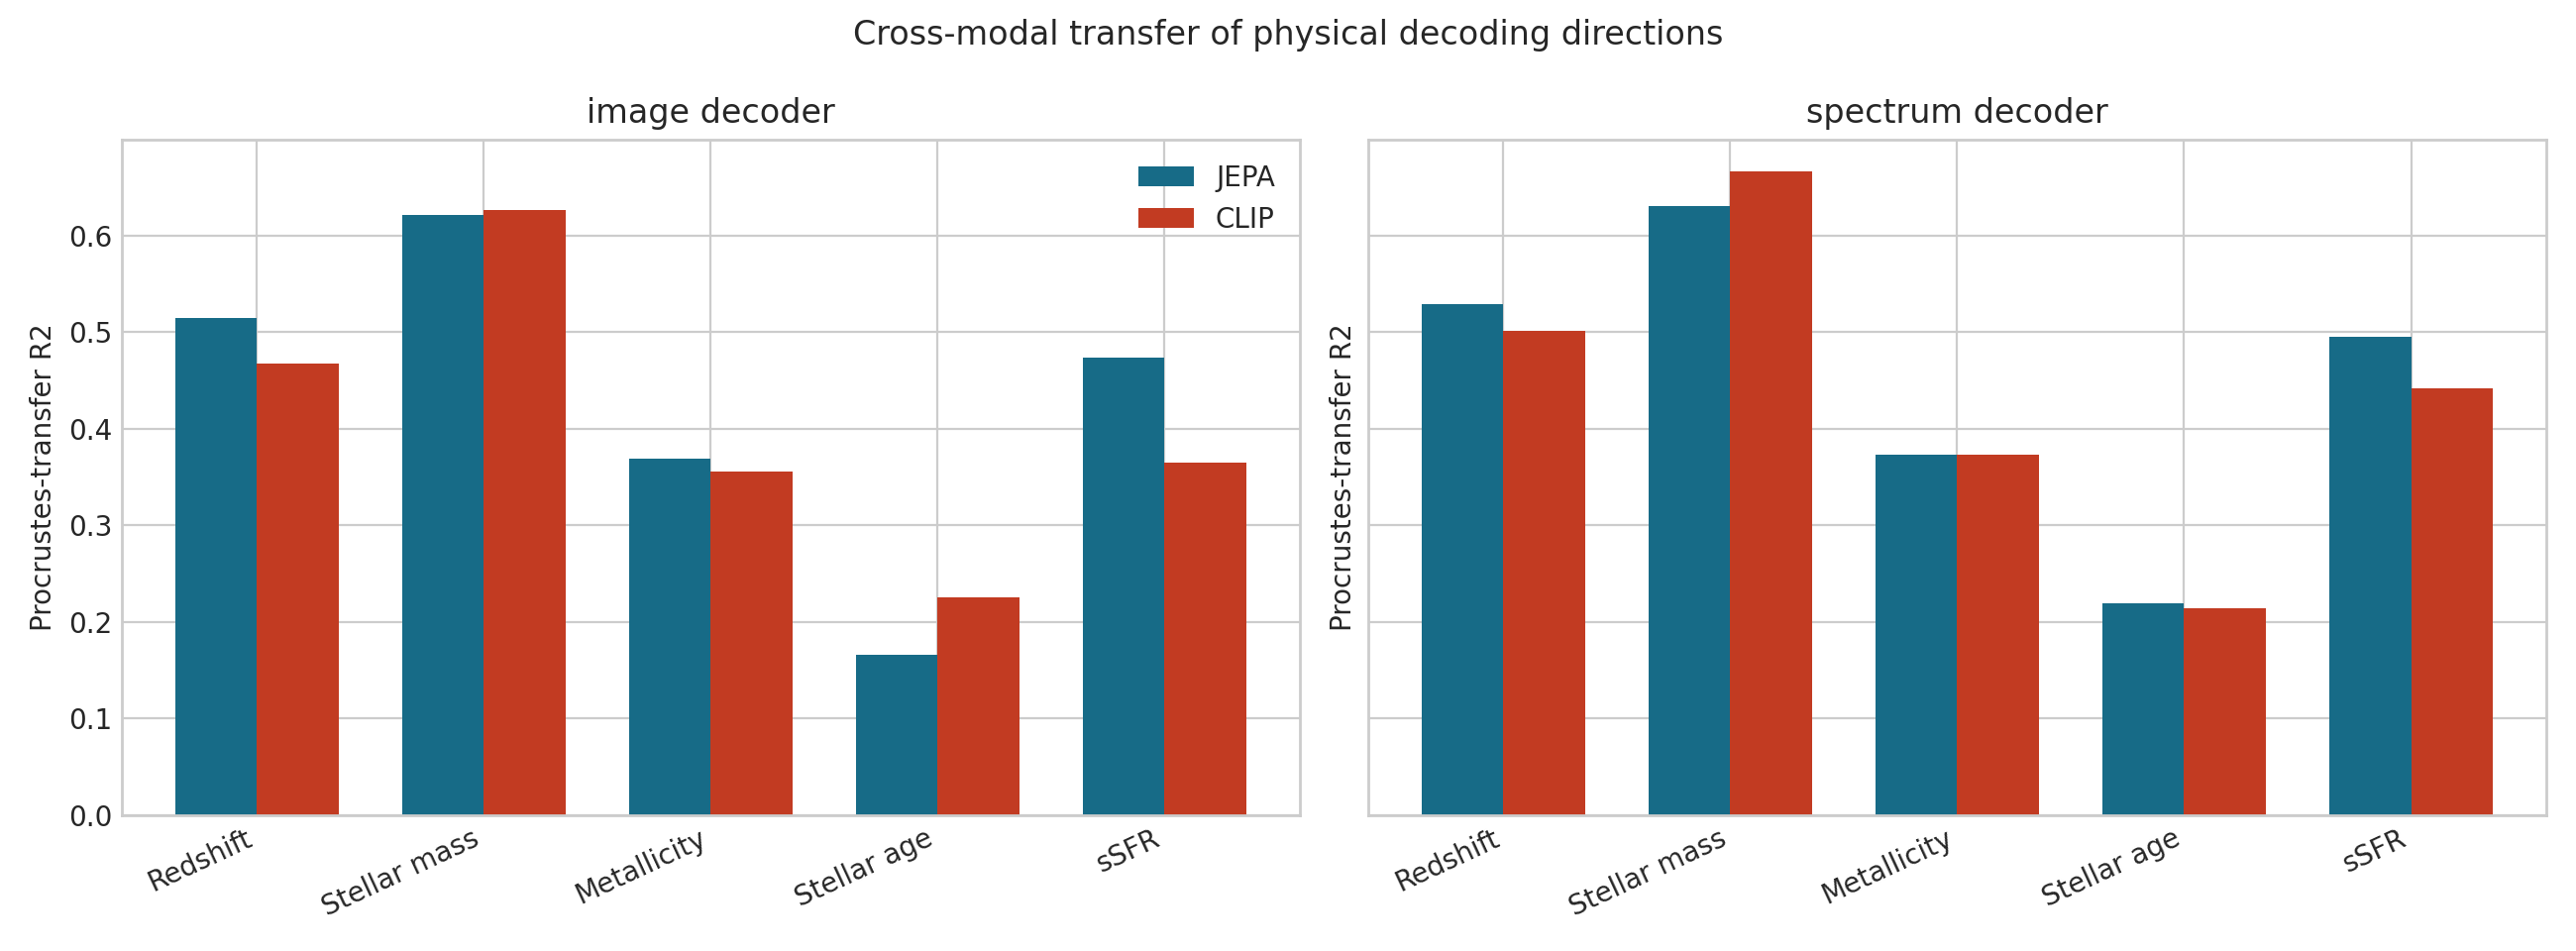
\includegraphics[width=\linewidth]{Figures/objectives/09_decoder_transfer.png}
\end{minipage}
\begin{minipage}{0.72\linewidth}
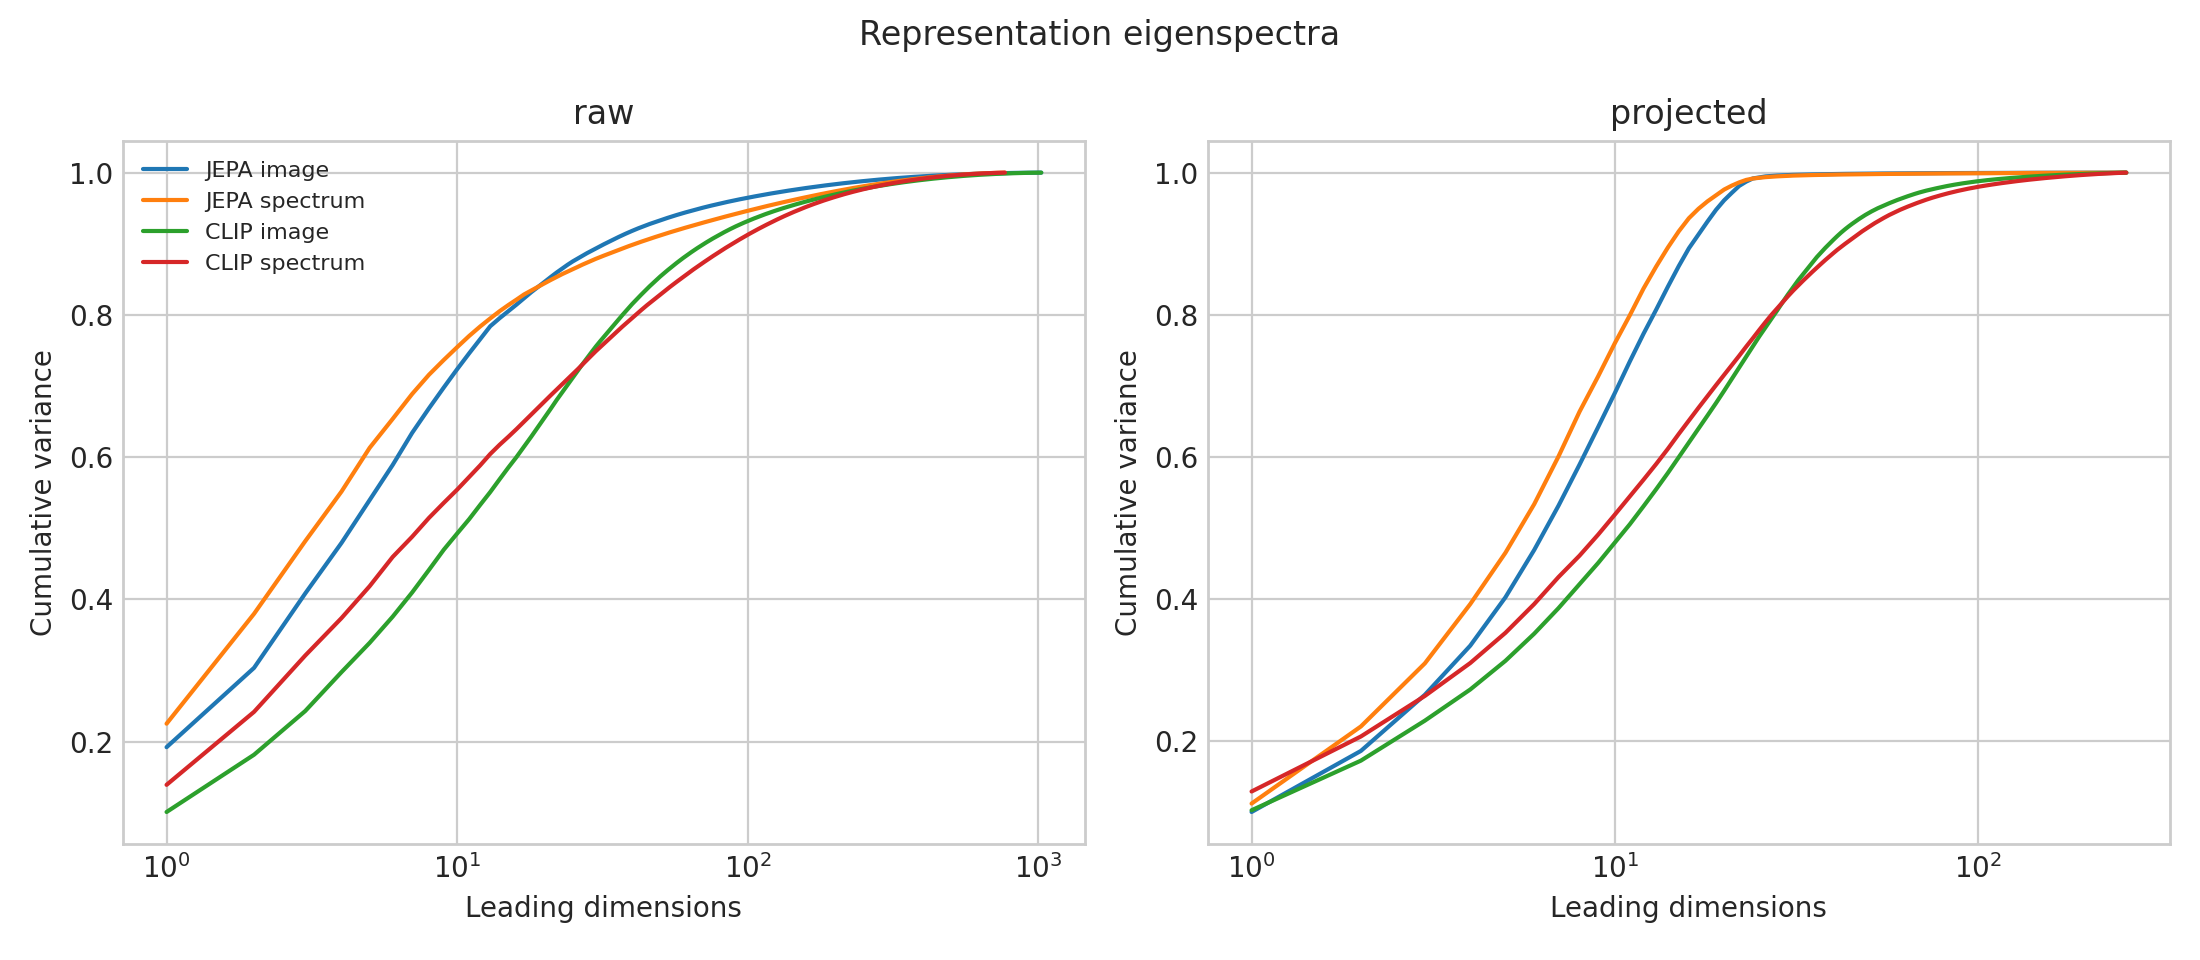
\includegraphics[width=\linewidth]{Figures/objectives/10_eigenspectra.png}
\end{minipage}
\caption{Additional objective diagnostics: raw/projected scientific probes,
Procrustes retrieval, decoder transfer (including own, direct, and aligned
scores), and covariance eigenspectra.}
\label{fig:objective_extra}
\end{figure}

\FloatBarrier
\section{Additional Downstream Results}
\label{app:downstream}

\subsection{Galaxy10 per-class behavior}

\begin{table}[h]
\centering
\caption{Per-class recall and F1 for the selected independent ViT-L/14
checkpoint.}
\label{tab:galaxy10_classes}
\small
\begin{tabular}{lrr@{\qquad}lrr}
\toprule
Class & Recall & F1 & Class & Recall & F1\\
\midrule
Disturbed & .486 & .457 & Merging & .771 & .762\\
Round smooth & .863 & .847 & In-between smooth & .786 & .794\\
Cigar smooth & .824 & .609 & Barred spiral & .628 & .643\\
Tight spiral & .652 & .634 & Loose spiral & .486 & .546\\
Edge-on, no bulge & .893 & .884 & Edge-on, bulge & .862 & .847\\
\bottomrule
\end{tabular}
\end{table}

Edge-on and smooth classes are strongest; disturbed and loose-spiral galaxies
remain difficult.
The model-selection curves and radar visualization appear in
Appendix~\ref{app:figures}.

\subsection{Galaxy Zoo DECaLS question-wise probes}

\begin{table}[h]
\centering
\caption{Public-split GZD-5 frozen-probe results for image SSL ViT-L/14 at 52k.
F1 is macro-F1 within each question.}
\label{tab:gzd5}
\small
\setlength{\tabcolsep}{4pt}
\begin{tabular}{lrrr@{\quad}lrrr}
\toprule
Question & Classes & Acc. & F1 & Question & Classes & Acc. & F1\\
\midrule
Smooth & 3 & .774 & .676 & Disk edge-on & 2 & .885 & .830\\
Spiral arms & 2 & .935 & .946 & Bar & 3 & .538 & .376\\
Bulge size & 5 & .776 & .762 & Roundedness & 3 & .825 & .825\\
Edge-on bulge & 3 & .800 & .711 & Spiral winding & 3 & .752 & .646\\
Arm count & 6 & .422 & .386 & Merging & 4 & .814 & .731\\
\midrule
\multicolumn{2}{l}{Question mean} & .752 & .689 &&&&\\
\bottomrule
\end{tabular}
\end{table}

The historical AstroCLIP context is 0.761 mean accuracy and 0.743 mean F1, but
its published head and evaluation details are not identical.
An early local reproduction also reached 0.761 accuracy but contained a
majority-class/protocol failure and is not used.
A stricter corrected variant measured $0.655\pm0.013$ mean F1.
We retain these variants to document protocol sensitivity rather than average
them into one headline number.

\subsection{Published context and comparability}

The independent image ViT-L's 71.83\% Galaxy10 accuracy is close to a 71.4\%
DINOv2 reference and below AION-1-L's 87.2\%; AION uses an MLP head and a much
larger multimodal corpus.
Likewise, recorded AstroCLIP spectrum values (redshift .98, mass .88, sSFR .64,
metallicity .58, age .43) use a different sample and training history.
Our scratch CLIP spectrum approaches several of these physical-property
numbers but not redshift.
These values provide context only and are not included in matched statistical
comparisons.

\clearpage
\section{Additional Figures and Qualitative Diagnostics}
\label{app:figures}

\begin{figure}[h!]
\centering
\begin{minipage}{0.49\linewidth}
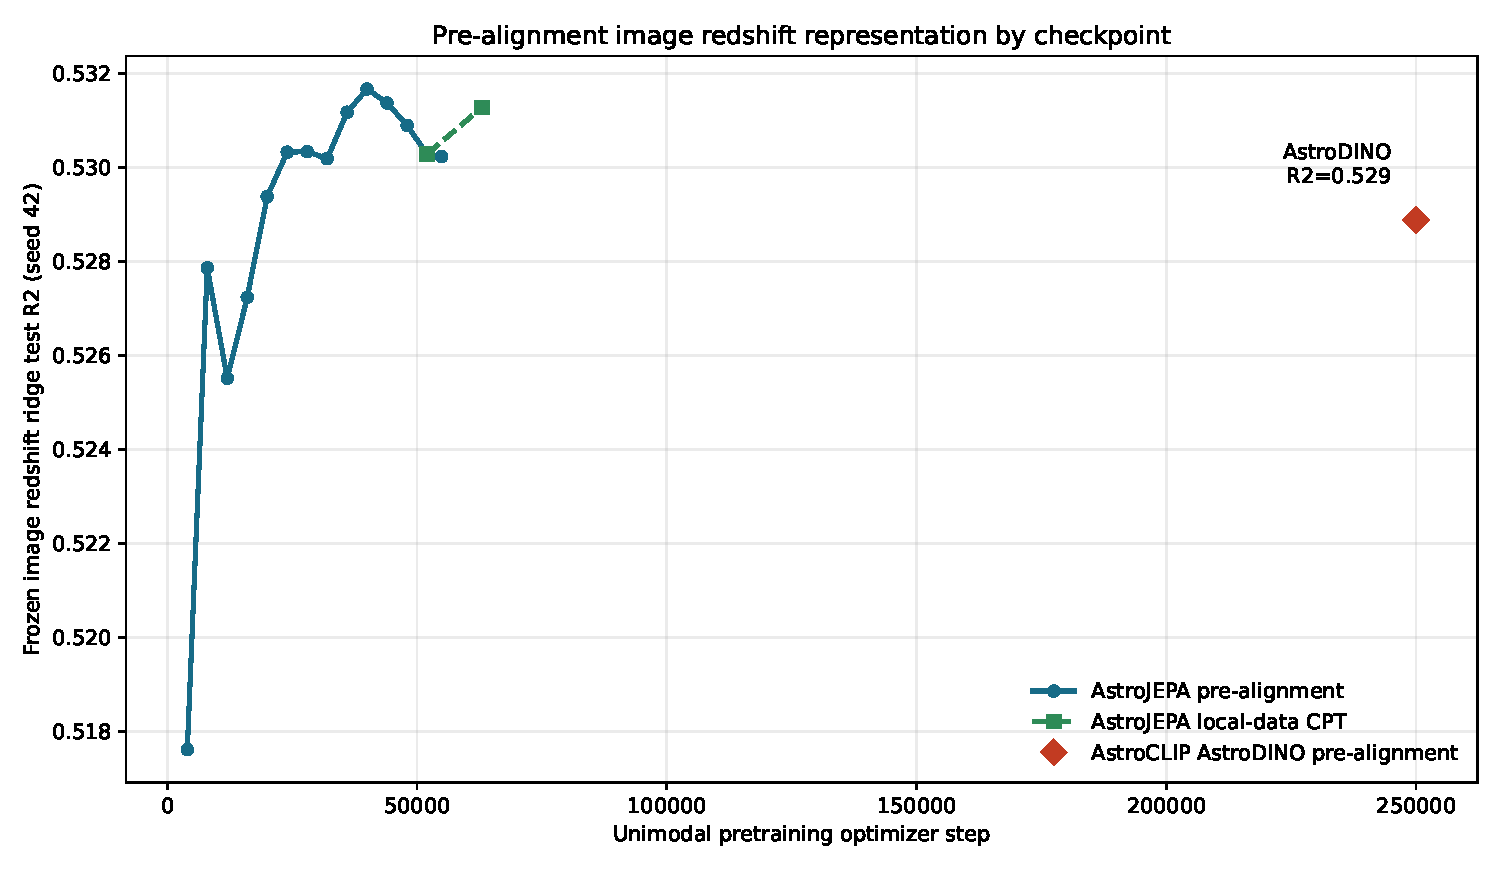
\includegraphics[width=\linewidth]{Figures/unimodal/image_redshift_step_vs_r2.pdf}
\end{minipage}
\begin{minipage}{0.49\linewidth}
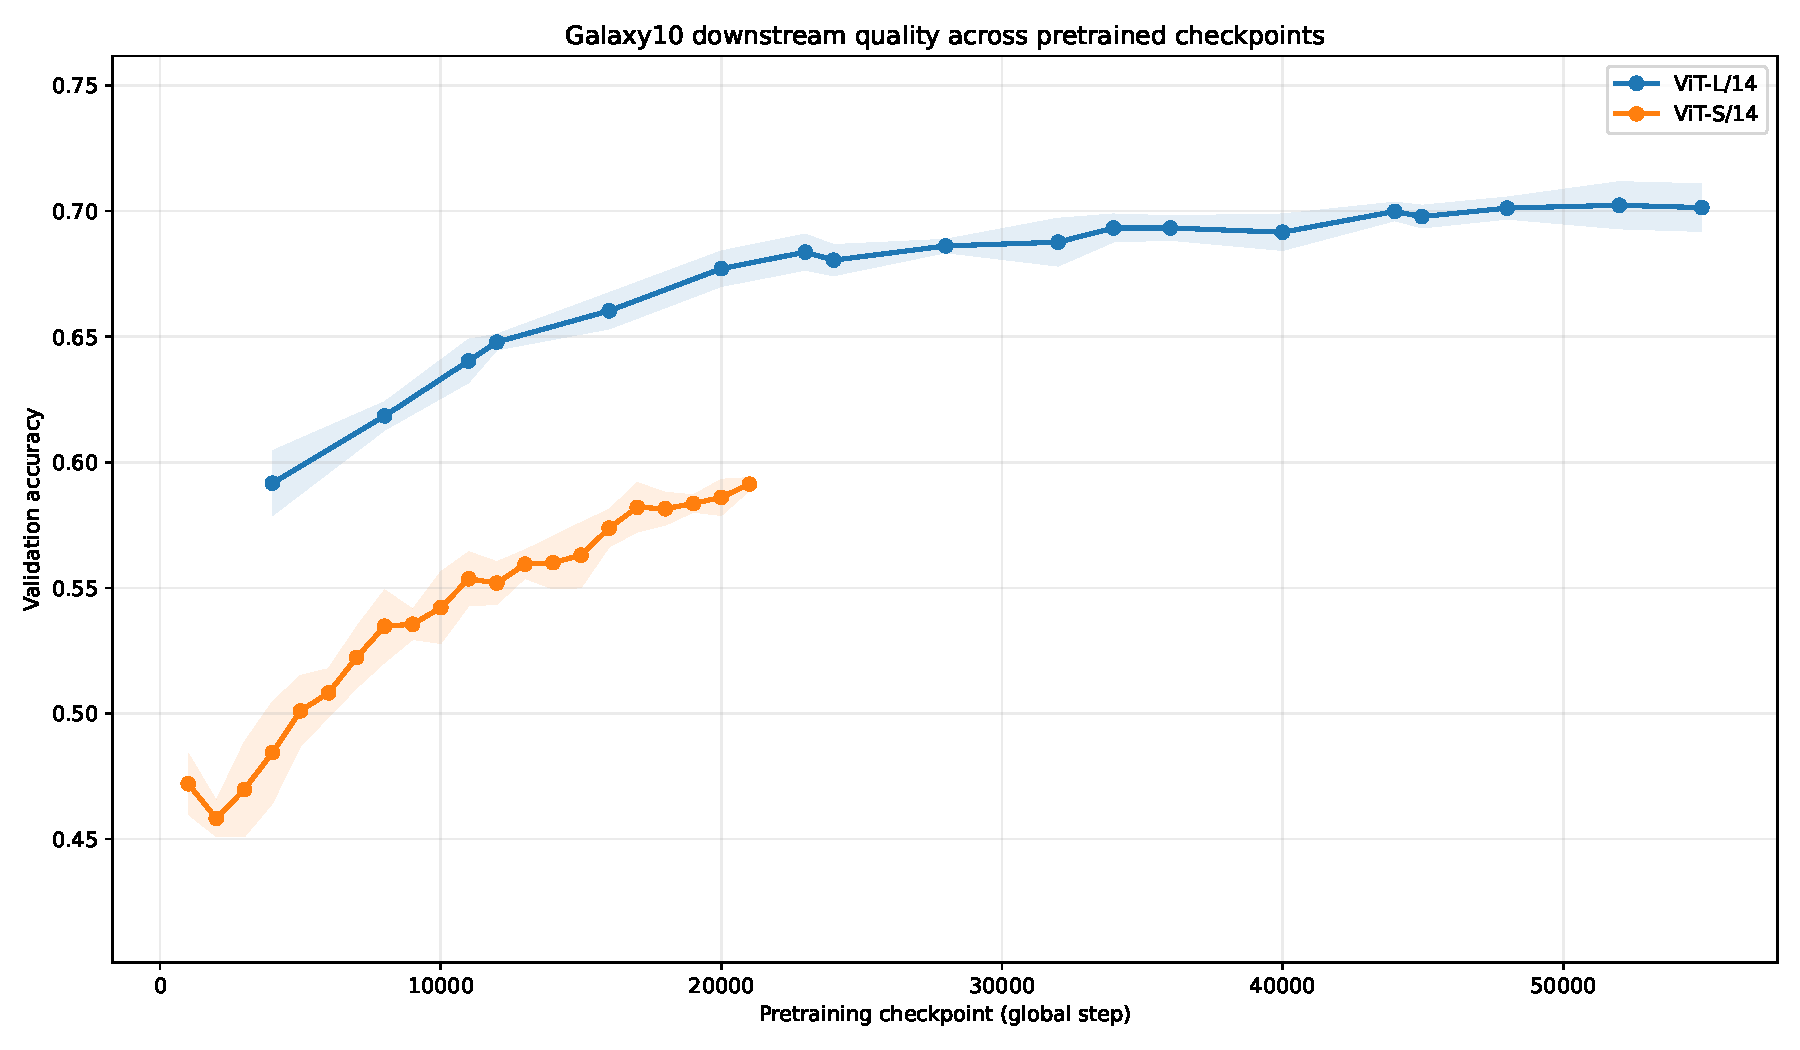
\includegraphics[width=\linewidth]{Figures/unimodal/all_models_validation_accuracy.pdf}
\end{minipage}
\begin{minipage}{0.49\linewidth}
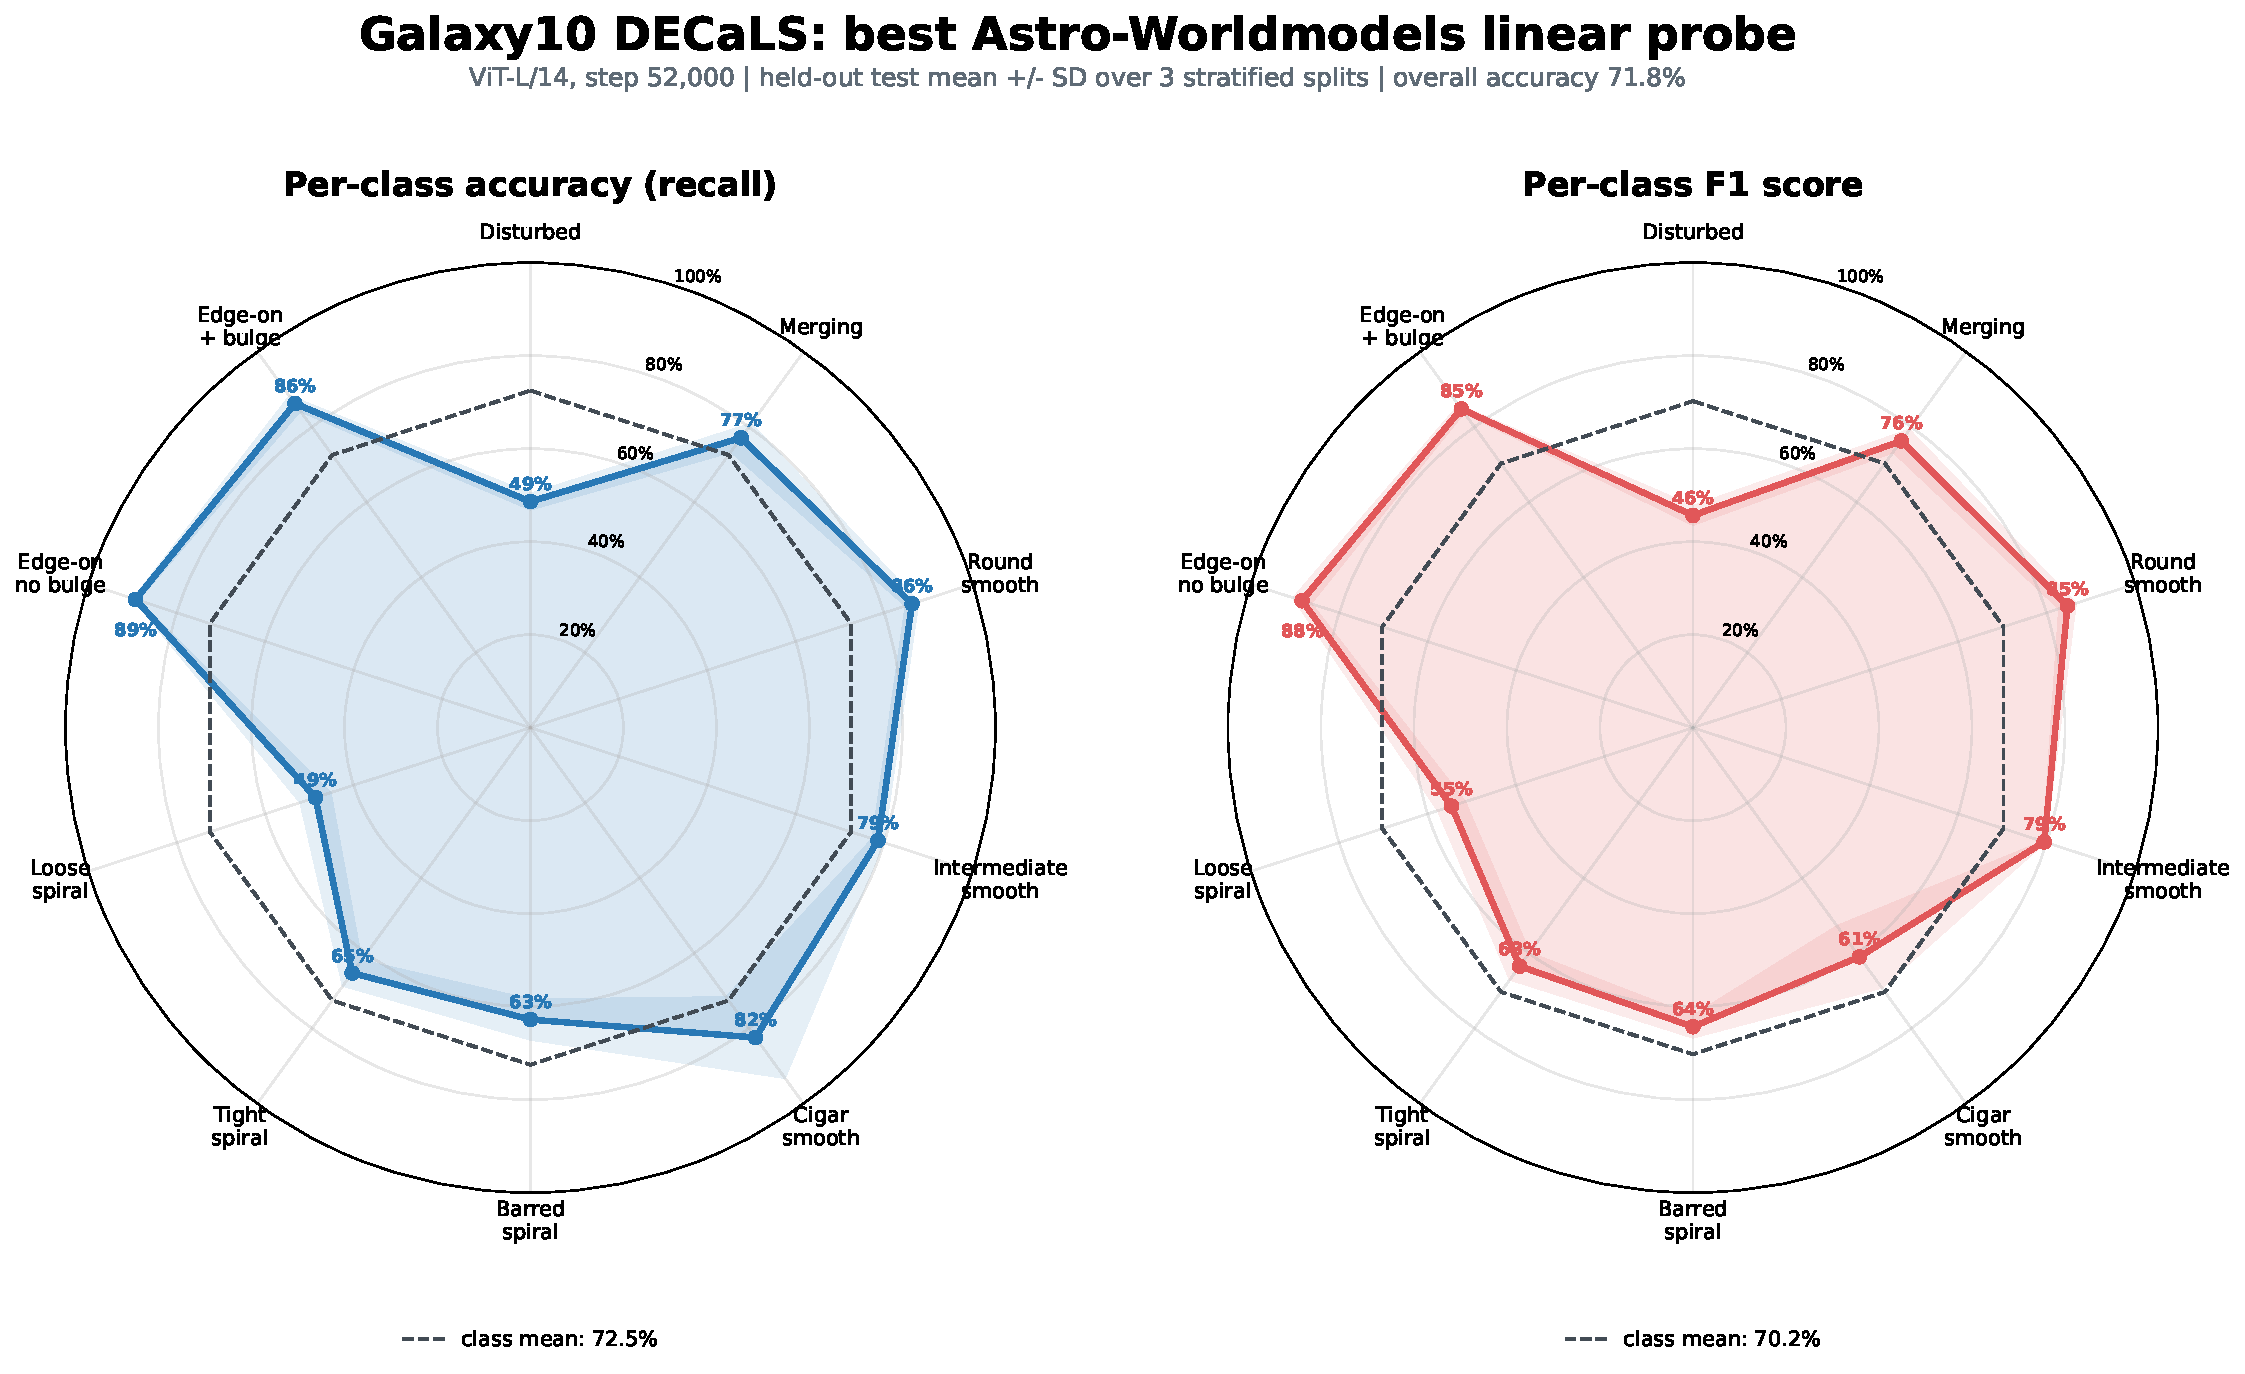
\includegraphics[width=\linewidth]{Figures/unimodal/best_model_galaxy10_per_class_radar.pdf}
\end{minipage}
\begin{minipage}{0.49\linewidth}
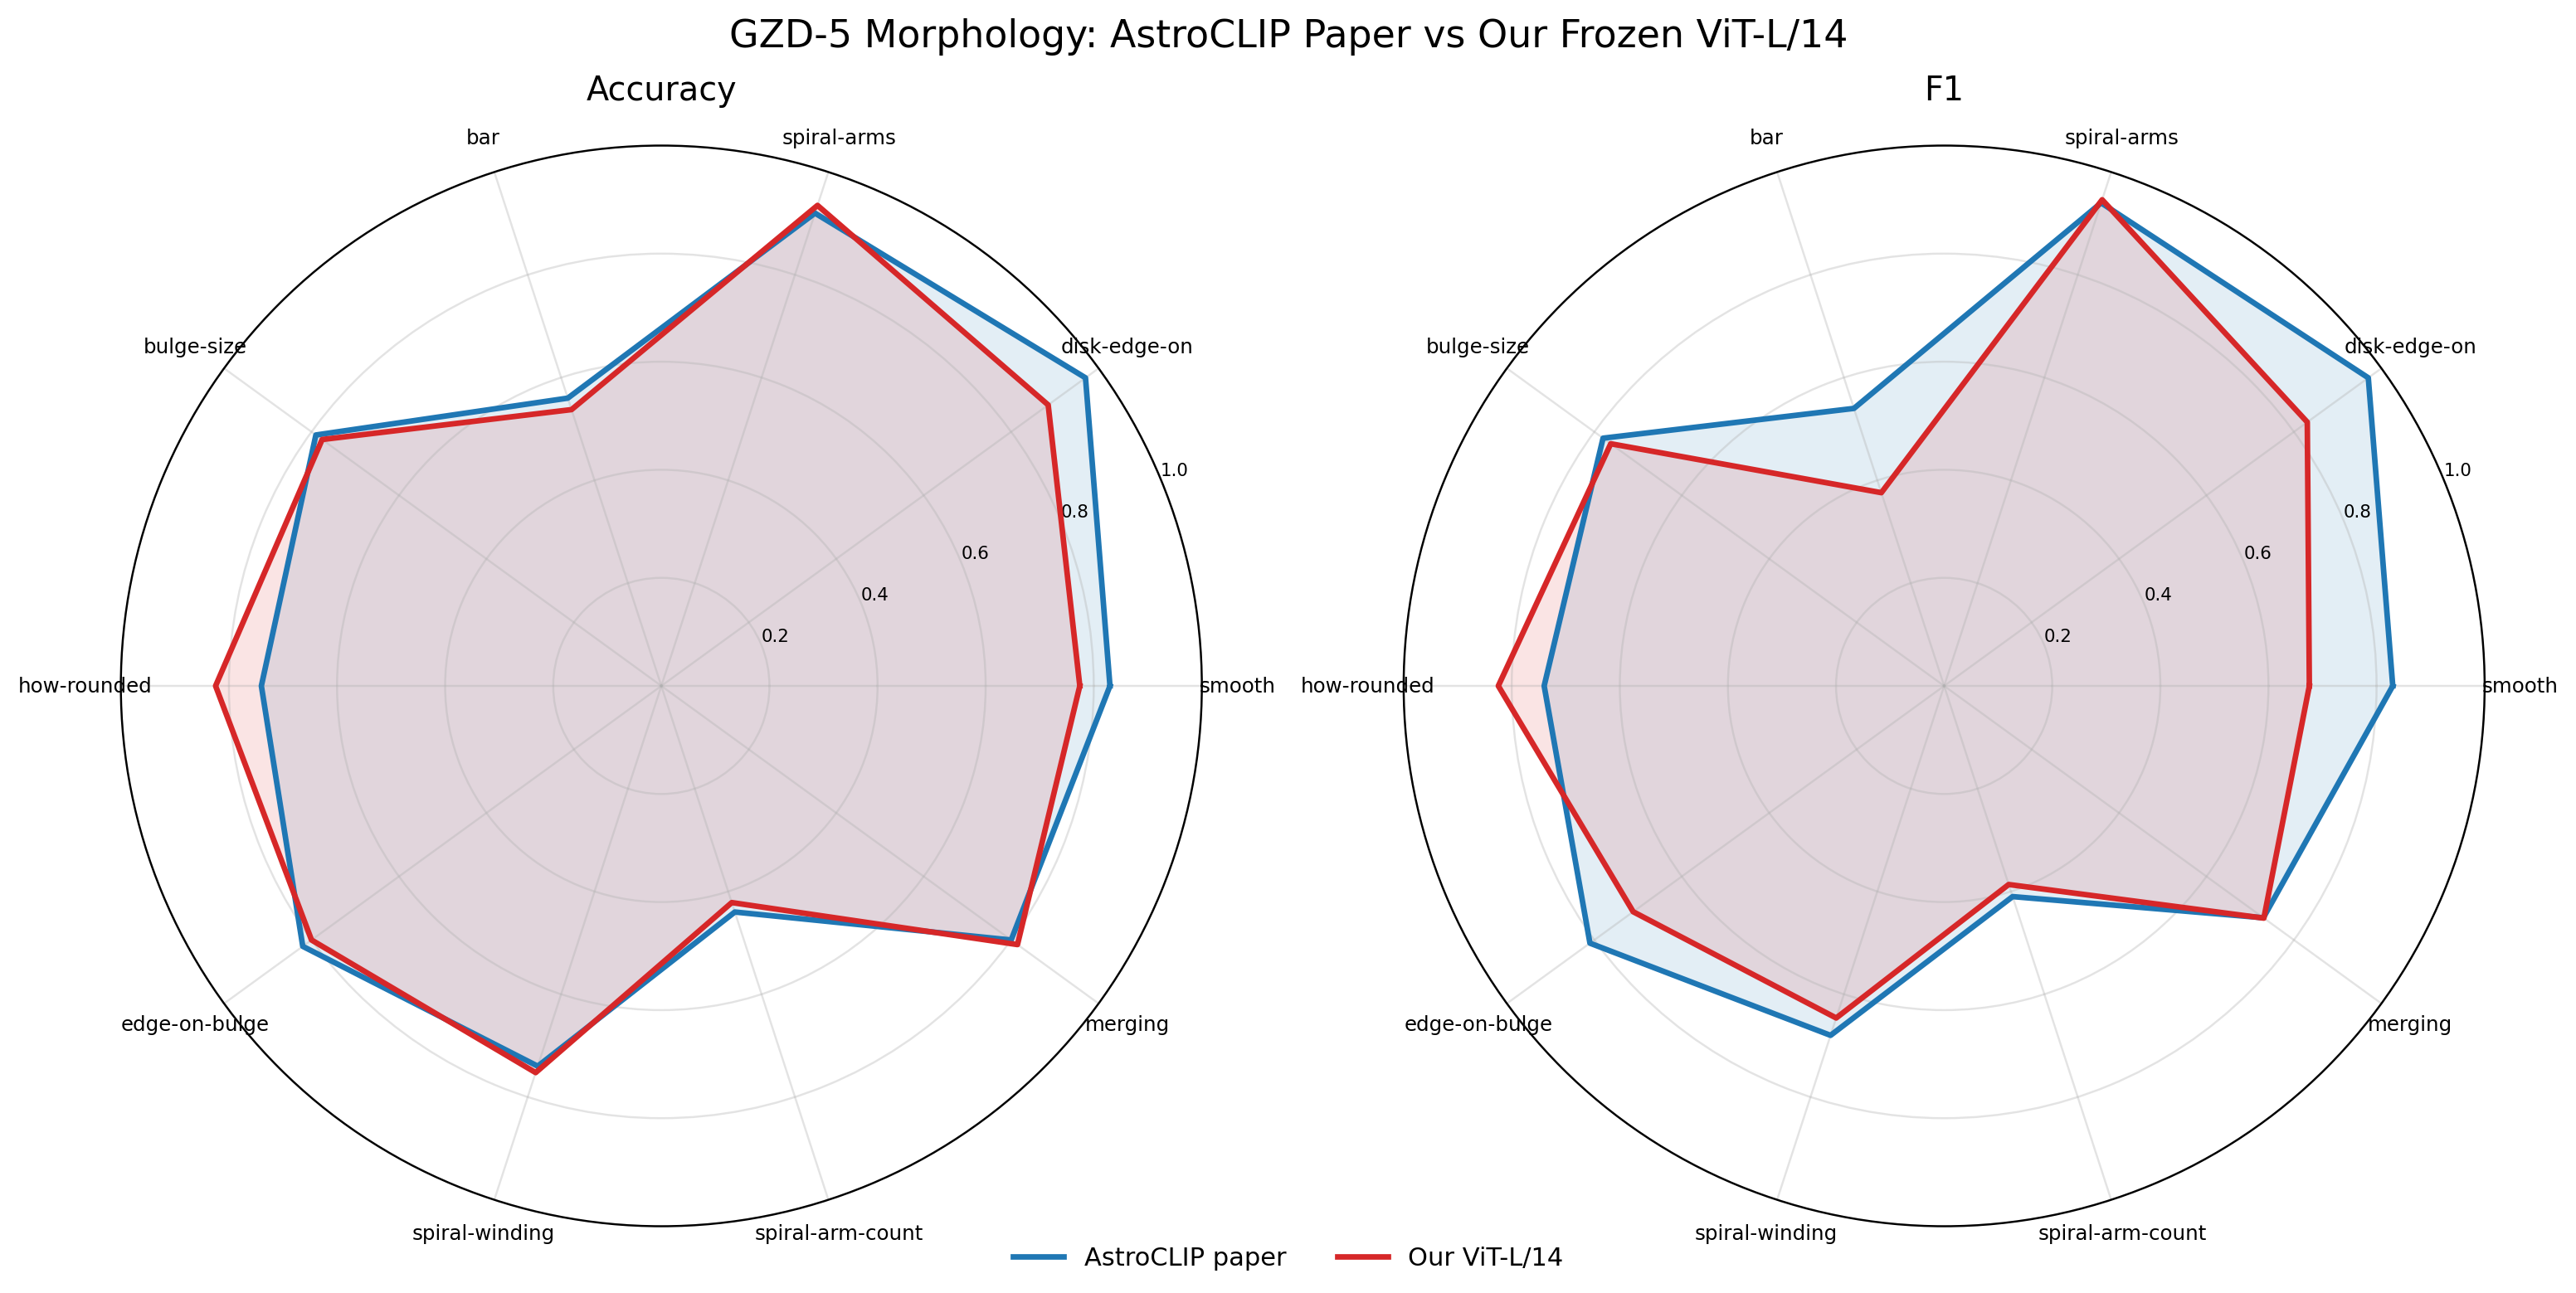
\includegraphics[width=\linewidth]{Figures/unimodal/astroclip_vs_ours_gzd5_radar.png}
\end{minipage}
\caption{Unimodal image evaluation: fixed-seed redshift progression, Galaxy10
checkpoint selection, selected-model per-class behavior, and public-split
GZD-5 context.}
\label{fig:unimodal_quant}
\end{figure}

\begin{figure}[p]
\centering
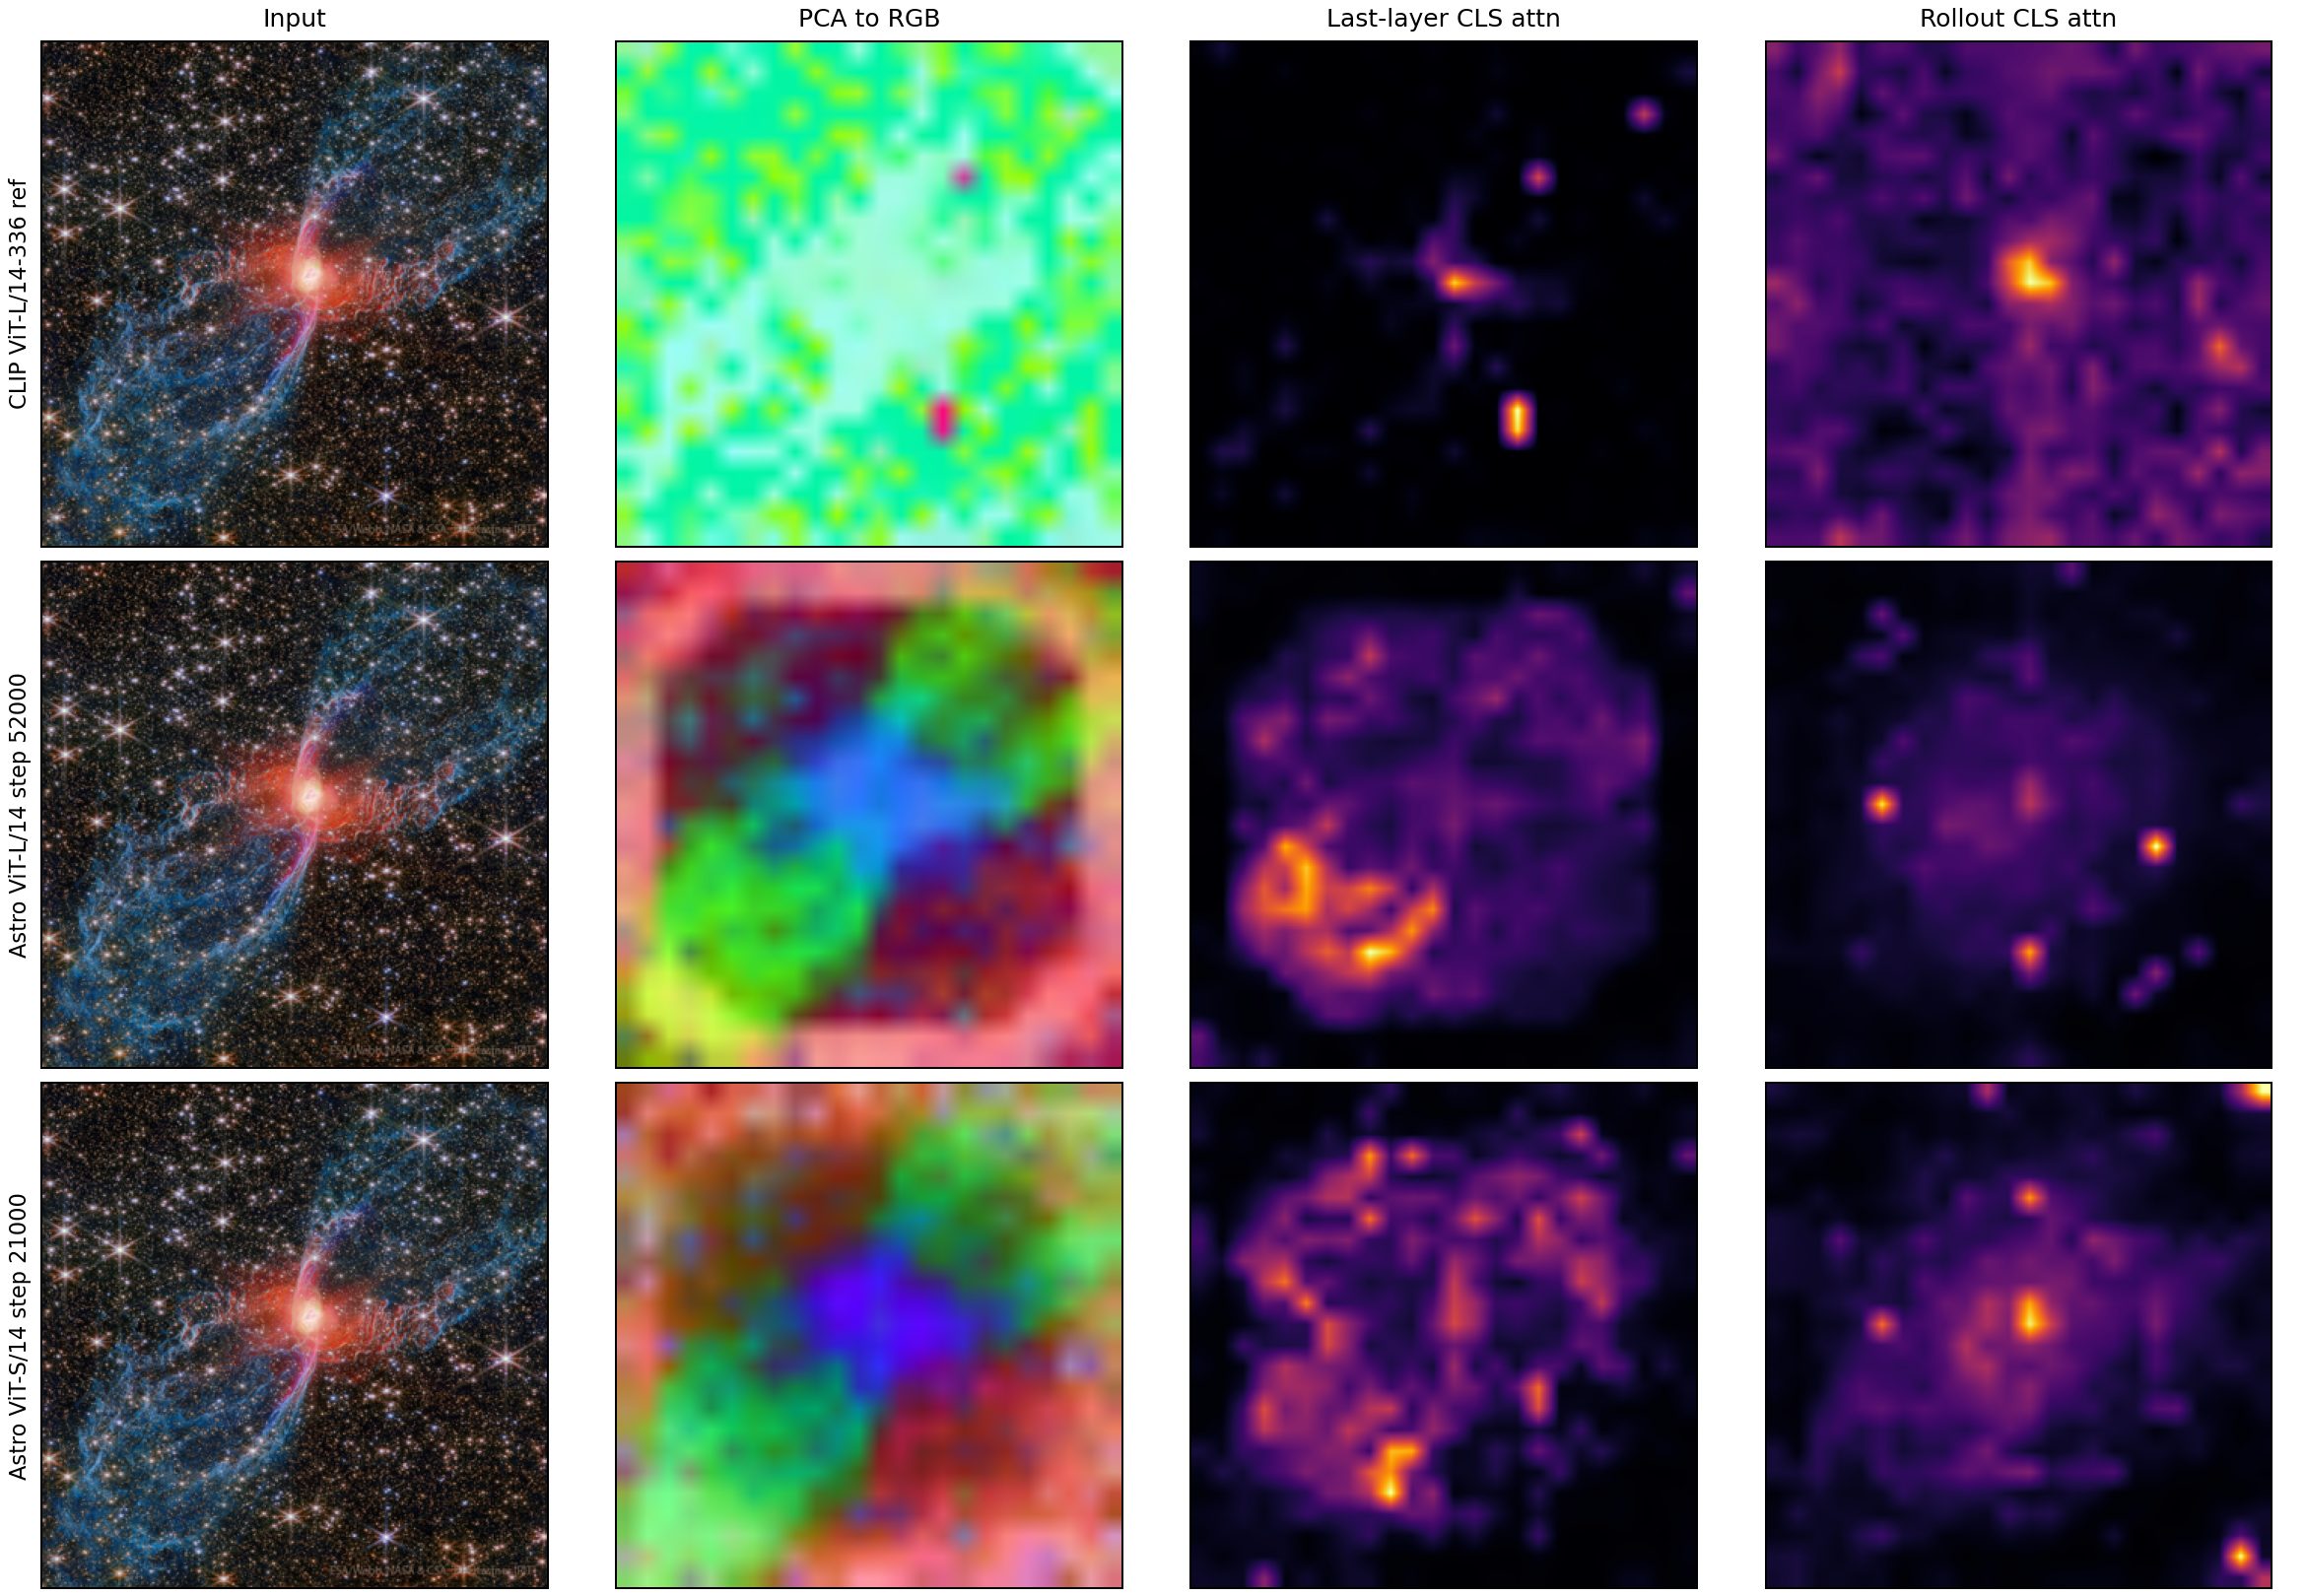
\includegraphics[width=.9\linewidth]{Figures/unimodal/comparison_grid.png}
\caption{Patch-token PCA and CLS-attention comparison for the selected
astronomy ViTs and reference image encoder.
These visualizations show structured, object-centered responses but are
qualitative diagnostics, not independent evidence for semantic localization.}
\label{fig:attention}
\end{figure}

\begin{figure}[p]
\centering
\begin{minipage}{0.49\linewidth}
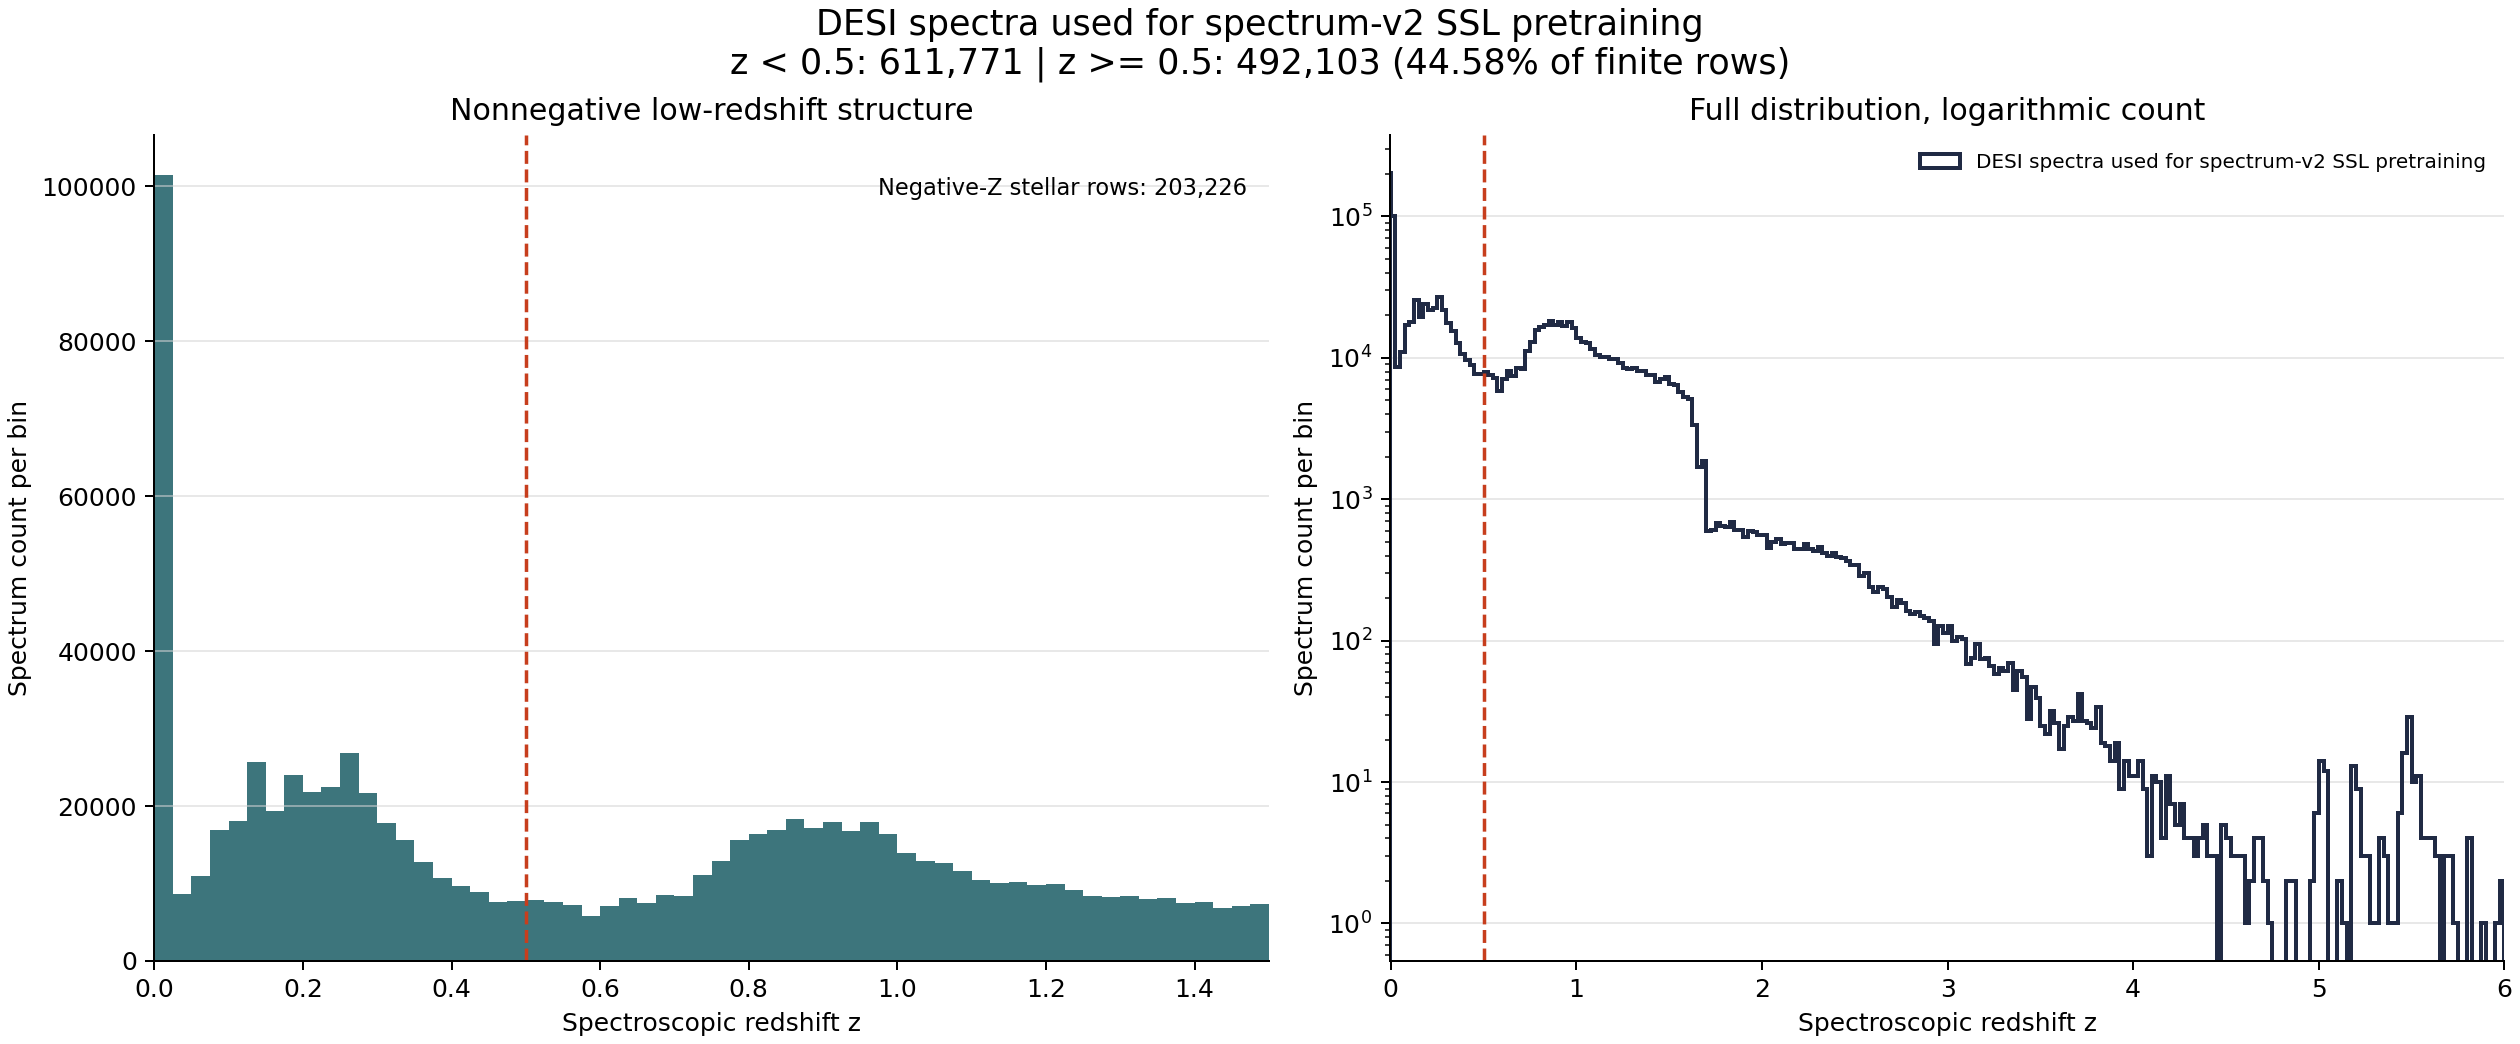
\includegraphics[width=\linewidth]{Figures/unimodal/ssl_pretraining_redshift_distribution.png}
\end{minipage}
\begin{minipage}{0.49\linewidth}
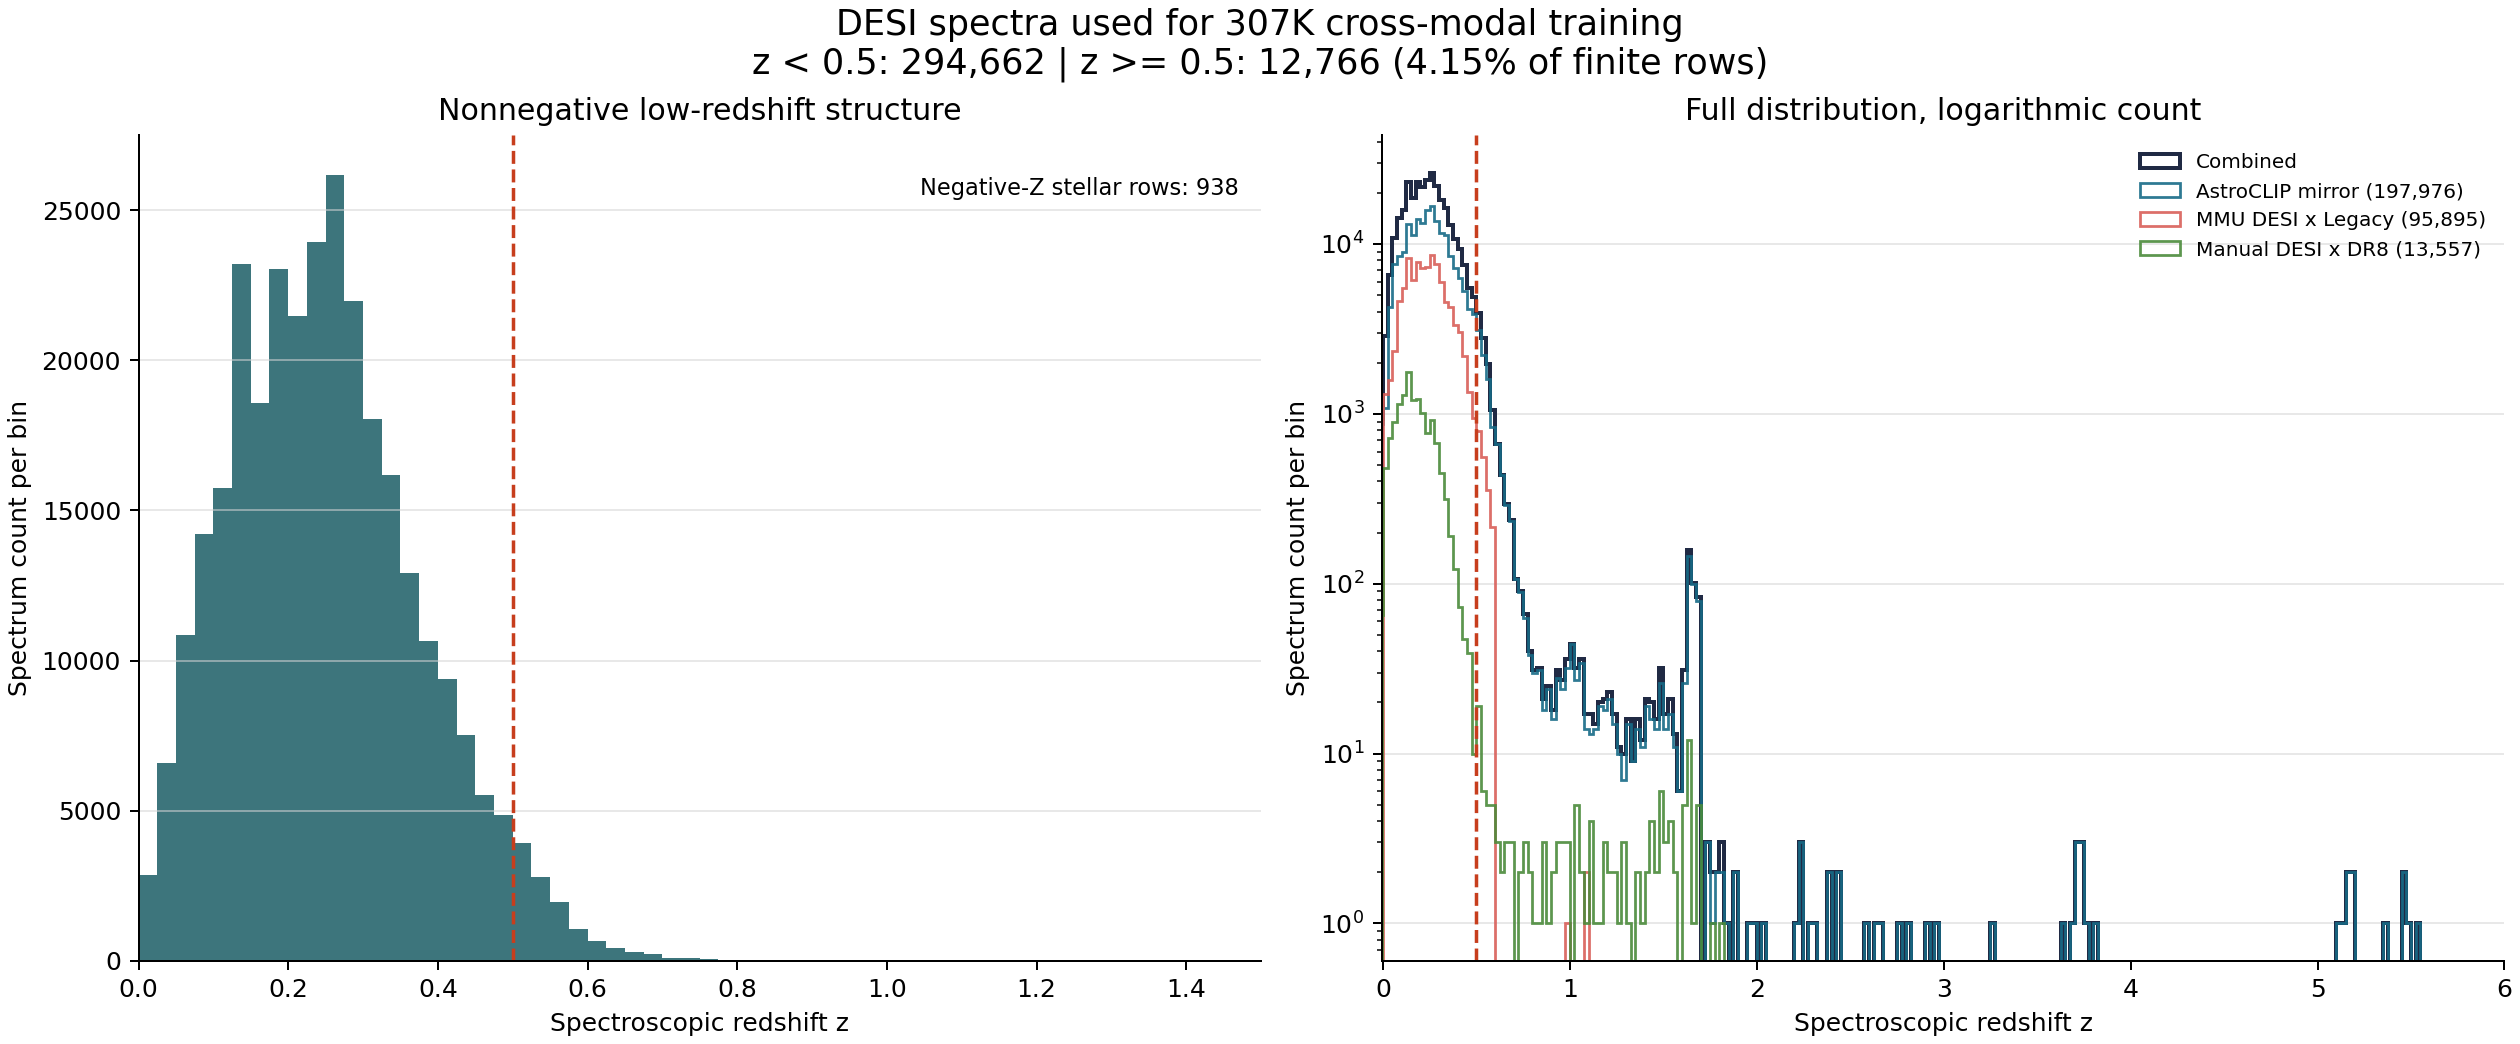
\includegraphics[width=\linewidth]{Figures/unimodal/crossmodal_redshift_distribution.png}
\end{minipage}
\caption{Redshift coverage differs sharply between spectrum SSL and paired
cross-modal training.
The spectrum SSL train set contains 492,103/1,103,874 (44.58\%) objects at
$z\geq0.5$, whereas the paired union contains 12,766/307,428 (4.15\%).
This shift is a plausible contributor to the cross-modal spectrum's redshift
behavior and limits generalization beyond the paired population.}
\label{fig:redshift_shift}
\end{figure}

\begin{figure}[p]
\centering
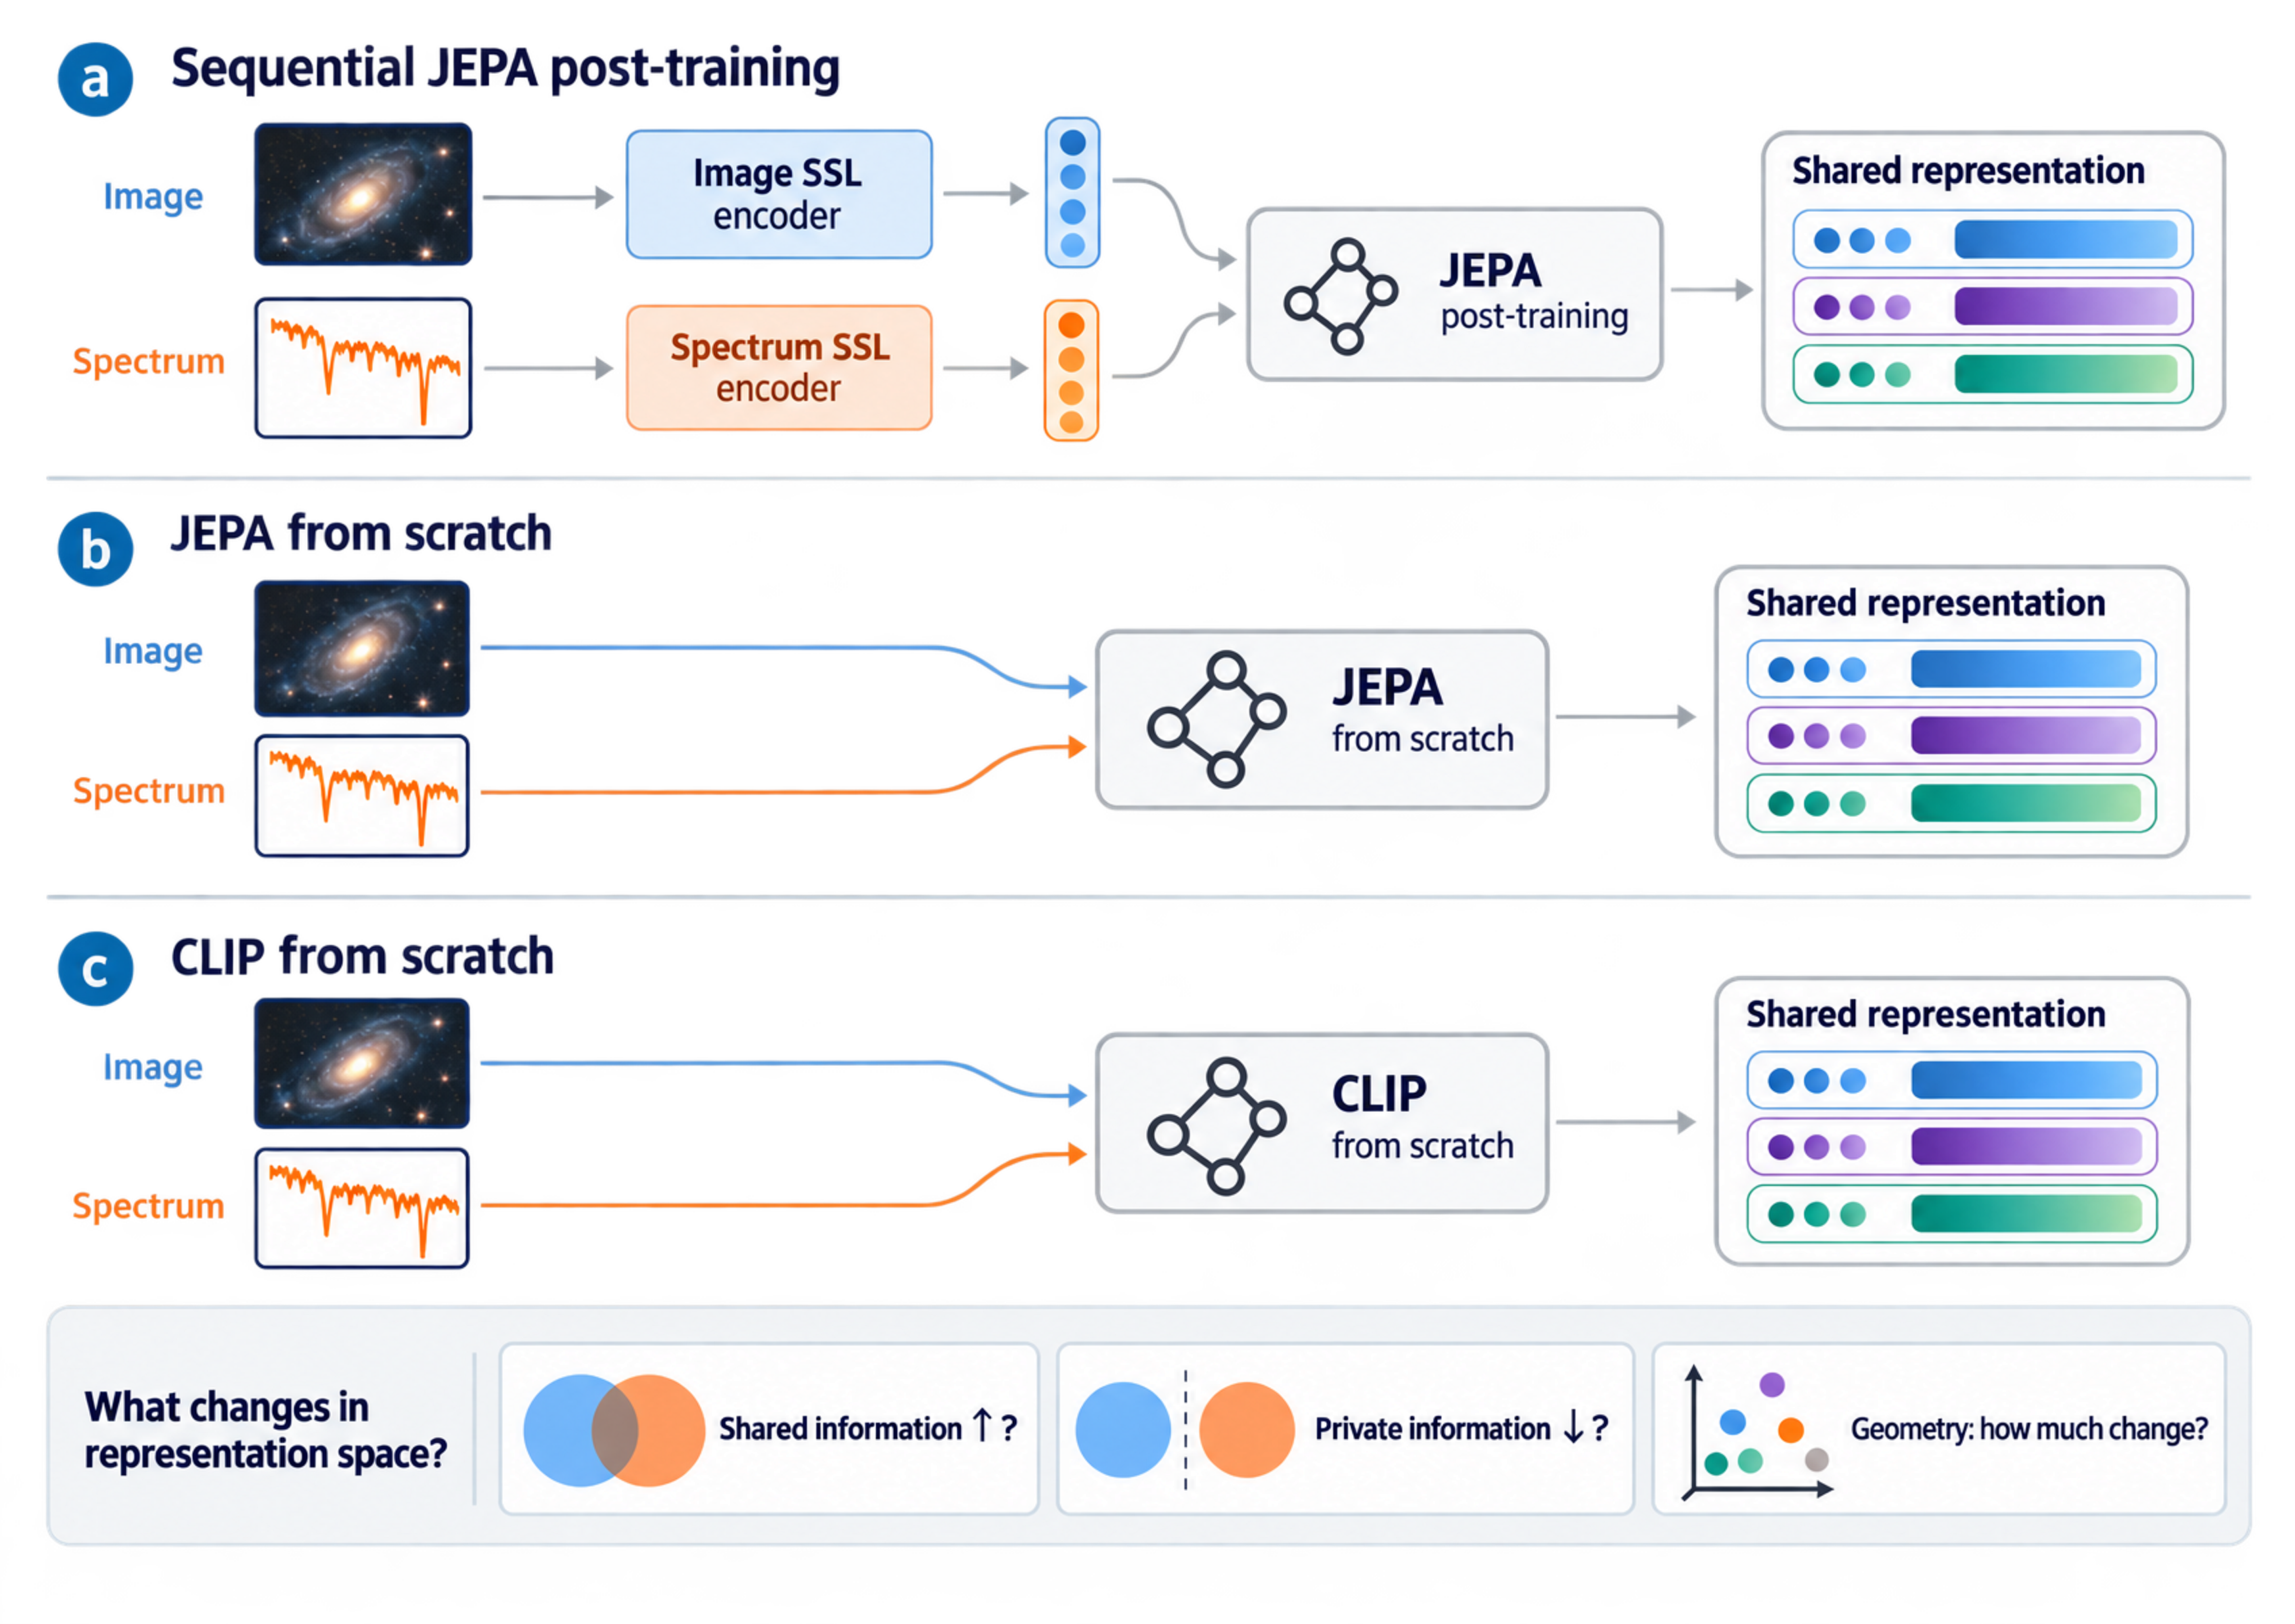
\includegraphics[width=.9\linewidth]{Figures/JEPA.png}
\caption{Expanded project schematic retained from the objective-comparison
study. It distinguishes sequential AstroJEPA, joint AstroJEPA, and a scratch
CLIP control, and motivates the shared/private/geometry diagnostics.
Figure~\ref{fig:architecture}, rather than this control-oriented diagram, is
the primary architecture figure.}
\label{fig:legacy_schematic}
\end{figure}

\FloatBarrier
\section{Additional Ablations, Null Results, and Reproducibility Inventory}
\label{app:ablations}

\subsection{Completed negative or qualified results}

\begin{itemize}
    \item \textbf{Image continuation pretraining:} one extra local-data epoch
    changes fixed-seed redshift \rscore\ from .53028 at the source checkpoint
    to .53128, insufficient evidence for a new scaling regime.
    \item \textbf{Spectrum v2 is not uniformly better:} it improves redshift,
    mass, metallicity, and age over v1 but changes sSFR from .510 to .496.
    \item \textbf{Objective heads are selective:} spectrum-v2 projected probes
    are uniformly below raw probes; joint shared states also trail raw states
    on most properties and sharply reduce Galaxy10 morphology.
    \item \textbf{Linear versus nonlinear probes:} a two-layer MLP materially
    improves joint-spectrum redshift and age, while the matched image MLP does
    not consistently improve on ridge.
    \item \textbf{Procrustes is insufficient:} orthogonal alignment improves
    retrieval only modestly for both JEPA+SIGReg and CLIP, ruling out a simple
    rotation as the entire cross-modal mismatch.
\end{itemize}

\subsection{Incomplete or invalid experiments}

\begin{table}[h]
\centering
\caption{Runs deliberately excluded from headline claims. Nothing in this table
is silently promoted to a completed result.}
\label{tab:incomplete}
\small
\begin{tabular}{p{0.32\linewidth}p{0.58\linewidth}}
\toprule
Experiment & Status and reason for exclusion\\
\midrule
First ViT-S prototype & checkpoint lineage/configuration was corrupt; not a
valid model comparison\\
First spectrum-v2 run & nominal epochs under-consumed rows because of double
worker sharding; replaced by corrected 172,390-update run\\
95k scratch AstroJEPA & useful feasibility pilot, but affected by the older
epoch-accounting loader; values are labeled as a pilot\\
Spectrum continuation pretraining & paused without a usable evaluation
checkpoint\\
No-SIGReg scratch control & not run; collapse prevention is therefore not an
empirical ablation in this study\\
Full pretrained fine-tuning & not run; prevents causal claims about
initialization versus scratch\\
Image local-token JEPA & designed/discussed but not trained\\
Spectrum-overlap audit & code path exists, but no complete result suitable for
reporting\\
SDSS/VIPERS extension & not run because wavelength grids, masks, resolution,
and selection were not yet harmonized\\
\bottomrule
\end{tabular}
\end{table}

\subsection{Artifact-to-claim map}

\begin{table}[h]
\centering
\caption{Repository experiment families audited for this manuscript.}
\label{tab:artifact_map}
\small
\begin{tabular}{>{\raggedright\arraybackslash}p{0.36\linewidth}>{\raggedright\arraybackslash}p{0.54\linewidth}}
\toprule
Artifact family & Paper disposition\\
\midrule
\path{Evals/cross_modal_backbone_eval} & final 307k probes,
95k pilot, nonlinear probes, checkpoint progression; Sections
\ref{sec:utility}, \ref{app:unimodal}, \ref{app:strategy}\\
\path{sequential vs joint} & central strategy study, all tables and five
summary figures; Section~\ref{sec:strategy}, Appendices
\ref{app:strategy}--\ref{app:representation}\\
\path{jepa vs clip} & controlled objective study, all ten figure families
and machine-readable tables; Appendix~\ref{app:clip}\\
\path{galaxy10_checkpoint_evolution} & model selection, uncertainty,
per-class results; Appendices~\ref{app:unimodal}, \ref{app:downstream},
\ref{app:figures}\\
\path{gzd5_morphology_probe} & public split plus protocol-sensitive
variants; Appendix~\ref{app:downstream}\\
\path{vit_patch_attention_diagnostics} & qualitative attention/PCA,
explicitly non-causal; Appendix~\ref{app:figures}\\
\path{spectra-redshift-diagnostics} & SSL-versus-paired distribution shift;
Appendix~\ref{app:figures}\\
\path{checkpoint_loss_curves} & training-health diagnostic; summarized,
not treated as a separate scientific result\\
\bottomrule
\end{tabular}
\end{table}

\paragraph{Statistical scope.}
Probe seeds quantify split/head variation, not representation-training
variation.
Retrieval and geometry metrics are deterministic over fixed representations.
The study has one principal representation-training seed per objective or
strategy, so no confidence interval should be interpreted as end-to-end model
uncertainty.

\paragraph{Reproducibility.}
The repository retains training entry points, frozen representation caches,
machine-readable JSON/CSV metrics, split metadata, checkpoint manifests,
figure-generation code, and study reports.
The paired loaders record source mixture, masks, and uncertainty availability;
checkpoints record source paths and training state.
Large datasets and checkpoints are not embedded in the paper directory.

\clearpage
\input{checklist_v2}

\end{document}
